\documentclass[12pt]{report}
\usepackage[top=2.5cm, bottom=2.5cm, left=4cm, right=2.5cm, centering, head=21.75 pt]{geometry}

\usepackage{amsmath}
\usepackage{amsthm}
\usepackage{subfigure}
\usepackage{booktabs}
\usepackage{caption}
\usepackage{amssymb}

\usepackage[italian]{babel}
\usepackage[utf8]{inputenc}
\usepackage{scrlayer-scrpage}
\ifoot[]{}
\cfoot[]{}
\ofoot[\pagemark]{\pagemark}
\pagestyle{scrplain}
\usepackage{mathptmx}
\usepackage{graphicx}
\usepackage{svg}
\usepackage{csquotes}
\usepackage[backend=biber, sorting=nty, ]{biblatex}
\appto{\bibsetup}{\raggedright}
\addbibresource{Thesis.bib}

\usepackage{titlesec}
\usepackage{float}

\usepackage{listings}
\renewcommand{\lstlistingname}{Code}
\usepackage{xcolor}
\definecolor{mygreen}{rgb}{0,0.6,0}
\definecolor{mygray}{rgb}{0.5,0.5,0.5}
\definecolor{mymauve}{rgb}{0.58,0,0.82}
\definecolor{darkgray}{rgb}{.4,.4,.4}
\definecolor{navy}{HTML}{000080}
\definecolor{purple}{rgb}{0.65, 0.12, 0.82}
\definecolor{codepurple}{rgb}{0.58,0,0.82}
\definecolor{backcolour}{rgb}{0.95,0.95,0.92}

\titleformat{\chapter}[block]
	{\normalfont\LARGE\bfseries}{\thechapter.}{0.5em}{\LARGE}
\titlespacing*{\chapter}{0pt}{-20pt}{25pt}

\usepackage{boxedminipage}
\usepackage{pgfplotstable}

\usepackage{times}

\begin{document}

	\begin{titlepage}
		\begin{center}
			{\LARGE{Università degli Studi di Milano Bicocca \\}}
			{\small{Dipartimento di Informatica, Sistemistica e Comunicazione}}\\
			{\small{Corso di Laurea Triennale}}
		\end{center}
			
		\begin{figure}[H]
			\centering
			%\includegraphics[width=0.4\textwidth]{Logo.png}
		\end{figure}

		\begin{center}
			{\Large { ??? }}
		\end{center}

		\vspace{2cm}

		\begin{minipage}[t]{0.47\textwidth}
			{\large{\bf Relatore:\\ XXX YYY}}
			\vspace{0.5cm}
			{\large{\bf \\Correlatore:\\ XXX YYY}}
		\end{minipage}\hfill\begin{minipage}[t]{0.47\textwidth}\raggedleft
			{\large{\bf Candidato: \\XXX YYY\\ }}
		\end{minipage}

		\vspace{25mm}

		\centering{\large{\bf ANNO ACCADEMICO 2023/2024 }}
	\end{titlepage}

	\tableofcontents
	\thispagestyle{empty}

	\listoffigures
	\thispagestyle{empty}
	\clearpage

	\setcounter{page}{1}

	\chapter{Abstract}

		Silhouette é una metrica spesso utilizzata per individuare
		la combinazione di iperparametri di un algoritmo di clustering
		non supervisionato che risulti nel clustering piú vicino possibile
		alla vera struttura di cluster dei dati in analisi. Verrá introdotta
		Silhouette e come calcolarla, alcune proprietá matematiche ed alcune
		applicazioni concrete su dataset di EHR (\textit{Electronic Health
		Records}). Verranno inoltre analizzati alcuni pacchetti per il
		linguaggio \texttt{R} che implementano Silhouette per determinare
		quale sia il migliore, comparandone le performance sia fra di
		loro sia rispetto all'implementazione di \texttt{scikit-learn}
		(\texttt{Python}).

	\chapter{Introduzione}

		Con il termine \textbf{cluster analysis}, o semplicemente
		\textbf{clustering}, si intende \emph{''una tecnica di
		classificazione statistica atta a scoprire se gli individui
		di una popolazione ricadono all'interno di certi gruppi mediante
		comparazioni quantitative di loro molteplici caratteristiche``}
		\footnote{\texttt{https://www.merriam-webster.com/dictionary/cluster\%20analysis}}.
		Informalmente, il clustering consiste nel (tentare di) suddividere
		un insieme di dati in gruppi, chiamati appunto \textbf{cluster},
		di modo che ciascun gruppo contenga elementi simili fra di loro
		ma dissimili rispetto a quelli degli altri gruppi.

		La definizione del concetto di ``somiglianza'' sta nelle mani di
		chi compie il clustering. In genere, l'analisi dei dati si occupa
		di dati numerici (altezze, lunghezze, età, ampiezze), pertanto il
		modo più naturale per formalizzare la somiglianza è dato da una
		\textbf{funzione di distanza}. Matematicamente, una qualsiasi
		funzione $d: \mathbb{R} \times \mathbb{R} \rightarrow \mathbb{R}$
		è considerabile una funzione di distanza se possiede (almeno) le
		seguenti proprietà:

		\begin{itemize}
			\item
			Per ogni $x \in \mathbb{R}$, $d(x, x) = 0$;
			\item
			Per ogni $x, y \in \mathbb{R}$, se $x \neq y$ allora $d(x, y) > 0$;
			\item
			Per ogni $x, y \in \mathbb{R}$, $d(x, y) = d(y, x)$
			(\textbf{simmetria});
			\item
			Per ogni $x, y, z \in \mathbb{R}$, $d(x, z) \leq d(x, y) + d(y, z)$
			(\textbf{disuguaglianza triangolare}).
		\end{itemize}

		Un \textbf{algoritmo di clustering} non é altro che un algoritmo
		che abbia in input un insieme di dati e che abbia in output il
		risultato del clustering. Algoritmi di questo tipo fanno uso di
		una funzione di distanza per raggruppare gli elementi in cluster
		senza che sia necessario farlo manualmente.

		Gli algoritmi di clustering si dividono in due macrocategorie:
		\textbf{algoritmi supervisionati} e \textbf{algoritmi non
		supervisionati}. Nei primi, viene usato un insieme di dati per
		generalizzarne le proprietá, cercando di predire il risultato
		per dati futuri, mentre nei secondi si cerca di catturare le
		proprietá dei dati in sé e per sé.

		Una volta applicato un algoritmo di clustering su un certo insieme
		di dati, é ragionevole chiedersi se il risultato del clustering
		effettivamente rispecchi la struttura dei dati o se l'algoritmo
		abbia errato. Negli algoritmi di tipo supervisionato questo é
		semplice, perché é possibile comparare i dati ottenuti con il
		risultato atteso, similmente a come viene fatto in un modello di
		regressione.

		Negli algoritmi di tipo non supervisionato questo é molto
		piú difficile, perché non c'é differenza fra l'insieme di
		dati utilizzato per costruire il modello e l'insieme di
		dati usato per testare il modello: sono lo stesso insieme.
		Una possibile soluzione al problema é data da delle statistiche,
		il cui valore rappresenta l'accuratezza del modello. Alcuni
		esempi sono: \textbf{Calinksi-Harabasz} \cite{Calinski01011974},
		\textbf{Davies-Bouldin} \cite{4766909} e \textbf{Dunn Index}
		\cite{Dunn01011974}.

		La statistica di interesse per questa tesi è Silhouette
		\cite{ROUSSEEUW198753}. Tale statistica, nelle parole
		dell'autore, si propone di rispondere alle seguenti domande:

		\begin{itemize}
			\item
			Il clustering è di buona qualità? In altre parole, gli elementi di
			uno stesso cluster sono fra di loro "vicini" ed al contempo "lontani"
			dagli elementi di tutti gli altri cluster?
			\item
			Quali sono gli elementi ben classificati, ovvero quelli che probabilmente
			si trovano nel cluster "giusto"?
			\item
			Quali sono gli elementi che è difficile stabilire con certezza in quali
			cluster vadano collocati, ovvero quelli che stanno "nel mezzo" fra più
			cluster?
			\item
			Il numero di cluster scelto è effettivamente rappresentativo del dataset
			o è 'artificioso'?
		\end{itemize}

		\begin{table}[h]
			\centering
			\footnotesize
			\begin{tabular}{| p{1.75cm} | p{1.75cm} | p{1.75cm} | p{1.75cm} | p{1.75cm} | p{1.75cm} |}
				\hline
				\multicolumn{6}{| p{12.5cm} |}{
					\textit{Identifying heterogeneous subgroups of systemic autoimmune
					diseases by applying a joint dimension reduction and clustering
					approach to immunomarkers} \cite{Chang2024}
				} \\
				\hline
				\textbf{Patologie} &
				\textbf{N. pazienti} &
				\textbf{Features} &
				\textbf{Algoritmi} &
				\textbf{Software} &
				\textbf{Metriche} \\
				\hline
				Lupus Eritematoso Sistemico, Artrite Reumatoide,
				Sindrome di Sjogren &
				11923 &
				biomarcatori (tradotti in variabili categoriali) &
				Multiple Correspondence Analysis K-means (clustering e dimensionality
				reduction insieme) &
				clustrd (R) &
				Silhouette \\
				\hline
				\multicolumn{6}{| p{12.5cm} |}{
					\textit{Association of comorbid-socioeconomic clusters with
					mortality in late onset epilepsy derived through unsupervised
					machine learning}
					\cite{Josephson_Gonzalez-Izquierdo_Engbers_Denaxas_Delgado-Garcia_Sajobi_Wang_Keezer_Wiebe_2023/10/01_2023}
				} \\
				\hline
				\textbf{Patologie} &
				\textbf{N. pazienti} &
				\textbf{Features} &
				\textbf{Algoritmi} &
				\textbf{Software} &
				\textbf{Metriche} \\
				\hline
				Epilessia (tardiva) &
				11307 &
				Fattori di rischio, comorbiditá (indice di Charlson) &
				Agglomerative Hierarchical Clustering &
				scikit-learn (Python), Python 3.6.3, Stata 16.1 &
				Silhouette, Davies-Bouldin \\
				\hline
				\multicolumn{6}{| p{12.5cm} |}{
					\textit{Exploration of critical care data by using unsupervised
					machine learning} \cite{HYUN2020105507}
				} \\
				\hline
				\textbf{Patologie} &
				\textbf{N. pazienti} &
				\textbf{Features} &
				\textbf{Algoritmi} &
				\textbf{Software} &
				\textbf{Metriche} \\
				\hline
				&
				1503 &
				Valori di test di routine di laboratorio (BUN, creatinina, glucosio, ...) &
				Kmeans &
				R 3.5.2 &
				Total within-cluster variation, Silhouette, Gap statistic \\
				\hline
				\multicolumn{6}{| p{12.5cm} |}{
					\textit{Identifying and evaluating clinical subtypes of Alzheimer’s
					disease in care electronic health records using unsupervised machine
					learning} \cite{Alexander2021}
				} \\
				\hline
				\textbf{Patologie} &
				\textbf{N. pazienti} &
				\textbf{Features} &
				\textbf{Algoritmi} &
				\textbf{Software} &
				\textbf{Metriche} \\
				\hline
				Malattia di Alzheimer &
				10065 &
				sintomi tipici, comorbiditá, dati demografici &
				K-Means, Kernel K-means, Affinity Propagation, Latent Class Analysis &
				&
				Silhouette, Coefficiente di Jaccard \\
				\hline
				\multicolumn{6}{| p{12.5cm} |}{
					\textit{Utilization of Deep Learning for Subphenotype Identification
					in Sepsis-Associated Acute Kidney Injury} \cite{01277230-202011000-00006}
				} \\
				\hline
				\textbf{Patologie} &
				\textbf{N. pazienti} &
				\textbf{Features} &
				\textbf{Algoritmi} &
				\textbf{Software} &
				\textbf{Metriche} \\
				\hline
				Sepsi &
				4001 &
				Segni vitali, test di laboratorio &
				K-Means &
				scikit-learn (Python), matplotlib (Python), SAS 9.4, R 3.4.3 &
				Silhouette, Davies-Bouldin, Calinksi-Harabasz \\
				\hline
			\end{tabular}
			\caption{Riassunto degli articoli scientifici che applicano Silhouette su EHR}
			\label{tbl:ehr}
		\end{table}

		\begin{table}[h]
			\centering
			\footnotesize
			\begin{tabular}{| p{3.25cm} | p{1.75cm} | p{2.5cm} | p{1.5cm} | p{1.5cm} |}
				\hline
				\multicolumn{5}{| p{12.5cm} |}{
					\textit{Silhouette Index as clustering evaluation tool}
					\cite{10.1007/978-3-030-52348-0_2}
				} \\
				\hline
				\textbf{Sintesi} &
				\textbf{Algoritmi} &
				\textbf{Dataset} &
				\textbf{Software} &
				\textbf{Metriche} \\
				\hline
				É possibile utilizzare Silhouette come "stopping rule" direttamente
				all'interno di un algoritmo di clustering? &
				RPCT &
				Dataset artificiale, generato mediante \texttt{cluster.Gen}, FCPS
				Dataset artificiale costituito da tre distribuzioni uniformi &
				clusterSim (R) &
				Adjusted Rand Index \\
				\hline
				\multicolumn{5}{| p{12.5cm} |}{
					\textit{Performance evaluation of the Silhouette index}
					\cite{10.1007/978-3-319-19369-4_5}
				} \\
				\hline
				\textbf{Sintesi} &
				\textbf{Algoritmi} &
				\textbf{Dataset} &
				\textbf{Software} &
				\textbf{Metriche} \\
				\hline
				Qual'é il modo corretto per calcolare la Silhouette media? &
				Complete-linkage, single-linkage &
				Quattro dataset artificiali con una struttura di cluster ben definita,
				\texttt{Iris}, \texttt{Wine} &
				&
				\\
				\hline
				\multicolumn{5}{| p{12.5cm} |}{
					\textit{A comparison of clustering quality indices using outliers and noise}
					\cite{doi:10.3233/IDA-2012-0545}
				} \\
				\hline
				\textbf{Sintesi} &
				\textbf{Algoritmi} &
				\textbf{Dataset} &
				\textbf{Software} &
				\textbf{Metriche} \\
				\hline
				Quali sono le prestazioni di Silhouette rispetto ad altre metriche? &
				K-means, model-based clustering, hierarchical clustering, algoritmo "random" &
				\texttt{clear} (struttura di cluster é ben definita),
				\texttt{out} (parte dei dati sono noise),
				\texttt{noi} (parte delle dimensioni sono noise) &
				&
				Calinski-Harabasz, C-index, Davies-Bouldin, Gamma, ARI \\
				\hline
				\multicolumn{5}{| p{12.5cm} |}{
					\textit{Condensed Silhouette: An Optimized Filtering Process for Cluster Selection in K-Means}
					\cite{NAGHIZADEH2020205}
				} \\
				\hline
				\textbf{Sintesi} &
				\textbf{Algoritmi} &
				\textbf{Dataset} &
				\textbf{Software} &
				\textbf{Metriche} \\
				\hline
				Nel caso di algoritmi di clustering partizionale, é possibile
				semplificare ulteriormente Silhouette? &
				K-Means &
				7 microarray gene expressions (migliaia di features), 7
				dataset reali famosi (come Iris) &
				Scikit-Learn (Python) &
				\\
				\hline
				\multicolumn{5}{| p{12.5cm} |}{
					\textit{CUBOS: An Internal Cluster Validity Index for Categorical Data}
					\cite{Gao2019CUBOSAI}
				} \\
				\hline
				\textbf{Sintesi} &
				\textbf{Algoritmi} &
				\textbf{Dataset} &
				\textbf{Software} &
				\textbf{Metriche} \\
				\hline
				É possibile estendere Silhouette per utilizzarla su valori discreti? &
				IDC &
				K-Modes &
				UCI &
				\\
				\hline
			\end{tabular}
			\caption{Riassunto degli articoli scientifici che studiano Silhouette da un punto di vista teorico}
			\label{tbl:theory}
		\end{table}

	\chapter{Metodi}

		\section{Silhouette}

			Si supponga di avere a disposizione un dataset di dimensione
			$N \times M$, dove $N$ indica il numero degli elementi e $M$ è
			il numero di attributi. Per comodità, si assuma che gli attributi
			siano tutti dati numerici (altezze, lunghezze, capacità, ecc...).
			Per ogni elemento, tutti i valori di ciascun attributo sono noti.

			A partire da tale dataset è possibile costruire quella che viene
			chiamata \textbf{matrice delle distanze}. Tale matrice ha dimensione
			$N \times N$ e, in ciascuna cella $(i, j)$, è presente un valore
			indicato con $d(i, j)$ che rappresenta il grado di "dissomiglianza"
			fra l'elemento $i$ e l'elemento $j$ del dataset.

			Tale grado di dissomiglianza è calcolato mediante una
			\textbf{funzione di distanza}, usando come input i valori
			degli attributi di $i$ e di $j$. Un esempio di funzione di
			distanza è la \textbf{distanza Euclidea}, definita come segue:

			\begin{equation}
				d(i, j) =
				\sqrt{\sum_{m = 1}^{M} (f_{i, m} - f_{j, m})^{2}} =
				\sqrt{(f_{i, 1} - f_{j, 1})^{2} + \dots +
					(f_{i, M} - f_{j, M})^{2}}
			\end{equation}

			Dove $f_{i, m}$ e $f_{j, m}$ indicano il valore del $m$-esimo
			attributo per, rispettivamente, l'$i$-esimo ed il $j$-esimo
			elemento del dataset.

			Altri esempi di distanze sono la \textbf{distanza di Manhattan}
			e la \textbf{distanza di Minkowski} (dal punto di vista di
			Silhouette, quale funzione di distanza venga usata è irrilevante).

			\begin{table}[h]
				\centering
				\pgfplotstabletypeset[
					col sep=comma,
					header=true,
					every head row/.style={before row=\toprule, after row=\midrule},
					every last row/.style={after row=\bottomrule},
					]{data/sdist.csv}
				\caption{Matrice delle distanze per il dataset \texttt{iris}. Per questioni
				di spazio sono presenti solamente i primi 6 elementi.}
				\label{tab:dist}
			\end{table}

			Una volta nota la matrice delle distanze, si supponga di applicare
			un algoritmo di clustering (K-Means, ad esempio) per suddividere il
			dataset in un certo numero di cluster, sia questo $K$. Per ciascun
			cluster, è interamente noto sia il numero di suoi elementi, sia
			a quale cluster ciascun elemento del dataset è stato assegnato.

			Per poter calcolare il coefficiente di Silhouette, è prima necessario
			introdurre due quantità per ciascun elemento $i$ del dataset, indicate
			rispettivamente con $a(i)$ e $b(i)$.

			Preso un elemento $i$ del dataset, sia $A$ il cluster in cui l'algoritmo
			lo ha riposto. Ammesso che $A$ contenga altri elementi all'infuori di $i$,
			è possibile definire $a(i)$ come distanza media fra $i$ e tutti gli elementi
			di $A$ escluso $i$ stesso:

			\begin{equation}
				a(i) = \frac{1}{|A| - 1} \sum_{j \in \{A - \{i\}\}} d(i, j)
			\end{equation}

			Tale valore misura quanto un cluster è \textit{coeso}, nel senso
			che se tale valore è piccolo per tutti gli elementi del cluster,
			questi si trovano fra loro vicini. Per tale motivo, $a(i)$ viene
			anche chiamata \textbf{distanza intra-cluster}.

			Dopodiché, in maniera simile, per un cluster $C$ diverso da $A$
			è possibile definire $D(i, C)$ come la distanza media fra $i$
			(che appartiene ad $A$) e gli elementi di $C$:

			\begin{equation*}
				D(i, C) = \frac{1}{|C|} \sum_{j \in C} d(i, j)
			\end{equation*}

			Tale valore misura quanto un cluster è \textit{separato}, nel senso
			che se tale valore è grande per tutti gli elementi del cluster a cui
			$i$ appartiene, il cluster nel suo complesso si trova molto distante
			da tutti gli altri. Per tale motivo $D(i, C)$ viene anche chiamata
			\textbf{distanza inter-cluster}.

			Assumendo che il numero di cluster sia più di uno, per uno stesso elemento
			$i$ è possibile calcolare la distanza inter-cluster per ogni possibile
			cluster $C$ distinto da $A$. Fra questi $K - 1$ cluster, è di particolare
			interesse il cluster che ha il più piccolo valore di distanza inter-cluster
			per $i$, chiamato \textbf{neighboring cluster}. Questo perché tale cluster
			è quello che, se il cluster $A$ non esistesse, sarebbe la miglior scelta
			per catalogare $i$, dato che è quello i cui elementi sono i più vicini ad
			$i$.

			Se il neighboring cluster per $i$ è il cluster $C'$, la distanza
			inter-cluster $D(i, C')$ viene indicata con $b(i)$:

			\begin{equation}
				b(i) = min_{C \neq A} D(i, C)
			\end{equation}

			Una volta calcolato $a(i)$ e $b(i)$ per l'elemento $i$ del dataset, è
			possibile assegnarvi un valore di Silhouette $s(i)$, così calcolato:

			\begin{equation}
				s(i) = \frac{b(i) - a(i)}{max\{a(i), b(i)\}}
			\end{equation}

			Se l'elemento $i$ si trova in un cluster che contiene solamente sé stesso,
			per convenzione il valore $s(i)$ viene posto a $0$ (è una scelta arbitraria,
			ma è anche quella più neutra).

			È facile verificare che, per qualsiasi elemento $i$:

			\begin{equation*}
				-1 \leq s(i) \leq 1
			\end{equation*}

			Si assuma infatti che $b(i) \geq a(i)$. L'espressione diventa:

			\begin{equation*}
				s(i) = \frac{b(i) - a(i)}{b(i)} =
				\frac{b(i)}{b(i)} - \frac{a(i)}{b(i)} =
				- \frac{a(i)}{b(i)}
			\end{equation*}

			Avendo assunto che $b(i)$ sia maggiore di $a(i)$, tale frazione è una
			frazione propria, e pertanto il suo valore è racchiuso nell'intervallo
			$[-1, 0]$.

			Si assuma invece $a(i) > b(i)$. L'espressione diventa:

			\begin{equation*}
				s(i) = \frac{b(i) - a(i)}{a(i)} =
				\frac{b(i)}{a(i)} - \frac{a(i)}{a(i)} =
				\frac{b(i)}{a(i)}
			\end{equation*}

			Avendo assunto che $a(i)$ sia maggiore di $b(i)$, tale frazione è una
			frazione propria, e pertanto il suo valore è racchiuso nell'intervallo
			$[0, 1]$.

			%Inoltre, $s(i)$ non varia se tutte le distanze vengono moltiplicate
			%per una costante $q$:
			%
			%\begin{equation*}
			%	s(i) = \frac{m b(i) - m a(i)}{max\{m a(i), m b(i)\}} =
			%	\frac{m(b(i) - a(i))}{m(max\{a(i), b(i)\})} =
			%	\frac{b(i) - a(i)}{max\{a(i), b(i)\}}
			%\end{equation*}

			\begin{table}
				\begin{boxedminipage}{0.25\linewidth}
						\pgfplotstabletypeset[
							col sep=comma,
							header=true,
							every head row/.style={before row=\toprule, after row=\midrule},
							every last row/.style={after row=\bottomrule},
						]{data/siOne.csv}
				\end{boxedminipage}
				\begin{boxedminipage}{0.25\linewidth}
						\pgfplotstabletypeset[
							col sep=comma,
							header=true,
							every head row/.style={before row=\toprule, after row=\midrule},
							every last row/.style={after row=\bottomrule},
						]{data/siTwo.csv}
				\end{boxedminipage}
				\begin{boxedminipage}{0.25\linewidth}
						\pgfplotstabletypeset[
							col sep=comma,
							header=true,
							every head row/.style={before row=\toprule, after row=\midrule},
							every last row/.style={after row=\bottomrule},
						]{data/siThree.csv}
				\end{boxedminipage}
				\caption{Valori di $s(i)$, cluster e neighboring cluster per
				i primi 10 elementi dei tre cluster. Si noti come i valori
				di $s(i)$ del primo cluster siano più alti ed il neighboring
				cluster sia sempre lo stesso, mentre gli altri due cluster
				hanno valori più variegati.}
				\label{tab:iris}
			\end{table}

			Per farsi una migliore idea del significato di $s(i)$, può essere
			utile considerare alcune situazioni estreme.

			Quando $s(i)$ è approssimativamente $1$ si ha che $b(i)$ è molto
			più grande di $a(i)$, e quindi la distanza fra $i$ ed i membri del
			cluster a cui appartiene è molto più piccola della distanza fra $i$
			ed i membri degli altri cluster. Questo significa che la scelta di
			aver posto $i$ in quel cluster è una buona scelta, perché persino
			la "seconda scelta" è di netto inferiore alla prima.

			Quando $s(i)$ è approssimativamente $0$ si ha che $b(i)$ e $a(i)$
			hanno lo stesso ordine di grandezza, e quindi la distanza fra $i$
			ed i membri del cluster a cui appartiene è comparabile a quella
			fra $i$ ed i membri del suo neighboring cluster. Questo significa
			che la scelta di aver posto $i$ in quel cluster è inconclusiva,
			nel senso che se fosse stato invece scelto il neighboring cluster
			si avrebbe avuto sostanzialmente lo stesso risultato.

			Quando $s(i)$ è approssimativamente $-1$ significa che $a(i)$ è molto
			più grande di $b(i)$, e quindi la distanza fra $i$ ed i membri del
			cluster a cui appartiene è molto più grande della distanza fra $i$
			ed i membri degli altri cluster. Questo significa che la scelta di
			aver posto $i$ in quel cluster è discutibile, perché vi sono cluster
			con cui $i$ ha più in comune rispetto a quello in cui si trova.

			%Altra interessante proprietà: spostando i nel suo neighboring cluster
			%il valore di $s(i)$ cambia di segno. Questo perché, molto banalmente,
			%le distanze rimangono le stesse ma i ruoli di $a(i)$ e $b(i)$ si invertono.

			I valori $s(i)$ non sono, di per loro, particolarmente informativi.
			È però possibile costruire un Silhouette plot di ciascun cluster
			come un bar chart dove ciascuna colonna $i$-esima ha altezza
			proporzionale a $s(i)$, ordinato dalla colonna più alta a quella
			più bassa. Tale grafico può essere arricchito riportando informazioni
			ulteriori per ciascun elemento come, ad esempio: in quale cluster si
			trova, qual'è il suo neighboring cluster, il suo valore di $s(i)$.

			\begin{figure}[h]
				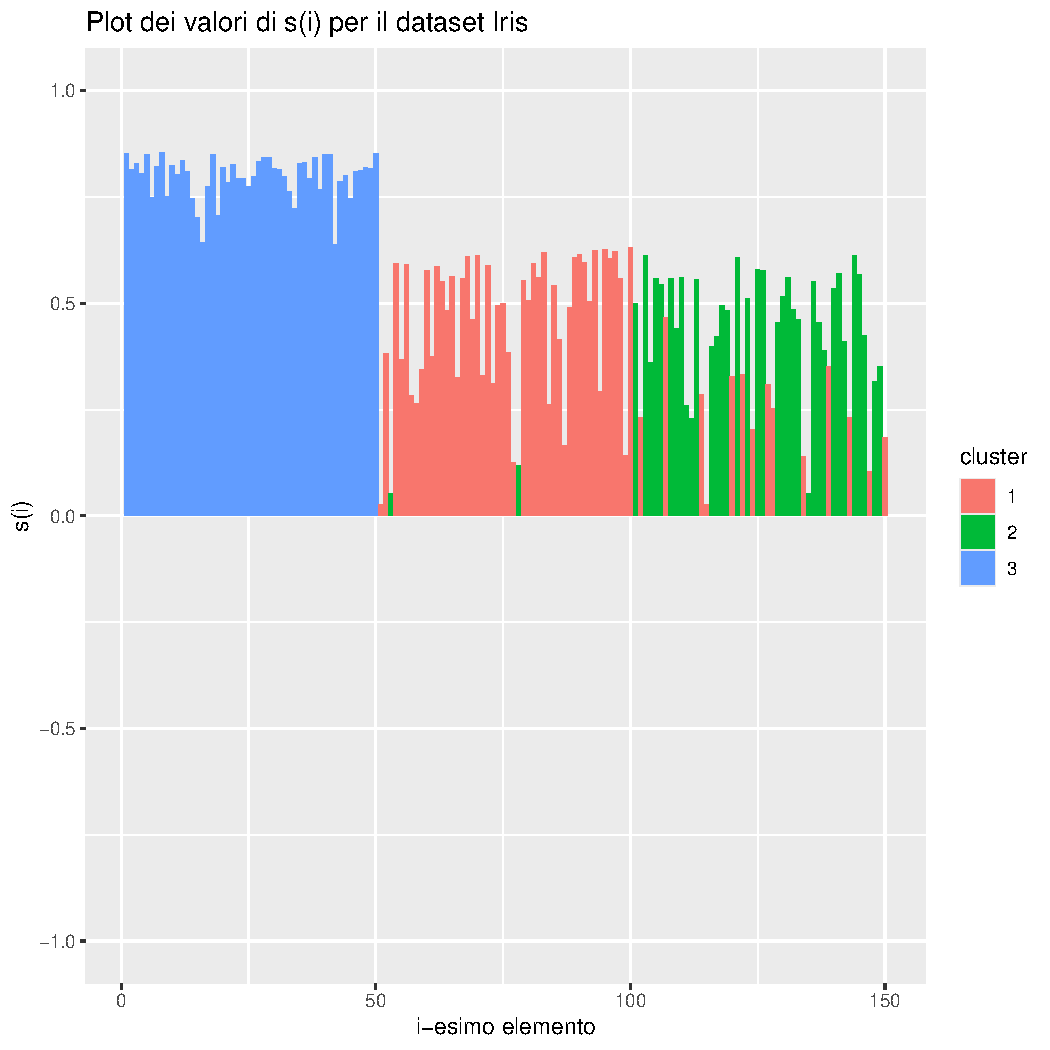
\includegraphics[width = \textwidth]{doc/si.pdf}
				\caption{Silhouette plot per il dataset \texttt{iris}.}
				\label{fig:si}
			\end{figure}

			Il vantaggio di Silhouette è che non dipende da quale algoritmo
			è stato usato per effettuare il clustering. Per tale motivo, può
			essere usato per valutare "a posteriori" il risultato dell'algoritmo,
			provando a modificare il valore degli iperparametri per valutare
			quale combinazione di iperparametri restituisce il risultato più
			coerente. Questo riesce particolarmente bene negli algoritmi in
			cui il numero di cluster figura fra gli iperparametri, come K-Means.

			Per esempio, si supponga che un dataset abbia effettivamente
			delle aree molto dense separate da aree ampie vuote. Operando
			un clustering in cui il numero di cluster è più basso del numero
			"naturale" di cluster, delle aree molto distanti tra loro vengono
			inglobate in un cluster unico nonostante vi siano considerevoli
			distanze nel mezzo. Silhouette può evidenziare questa situazione
			perché il valore di $a(i)$ tende ad essere molto alto, essendo
			i membri del dataset molto distanti dai loro centroidi.

			Si supponga invece di operare un clustering in cui il numero
			di cluster è più alto del numero "naturale" di cluster. In tale
			situazione, anche aree dense vengono spezzate in cluster diversi.
			Silhouette può evidenziare questa situazione perché il valore di
			$b(i)$ tende ad essere molto basso, dato che elementi molto vicini
			vengono separati forzosamente.

			\begin{figure}[h]
				\centering
				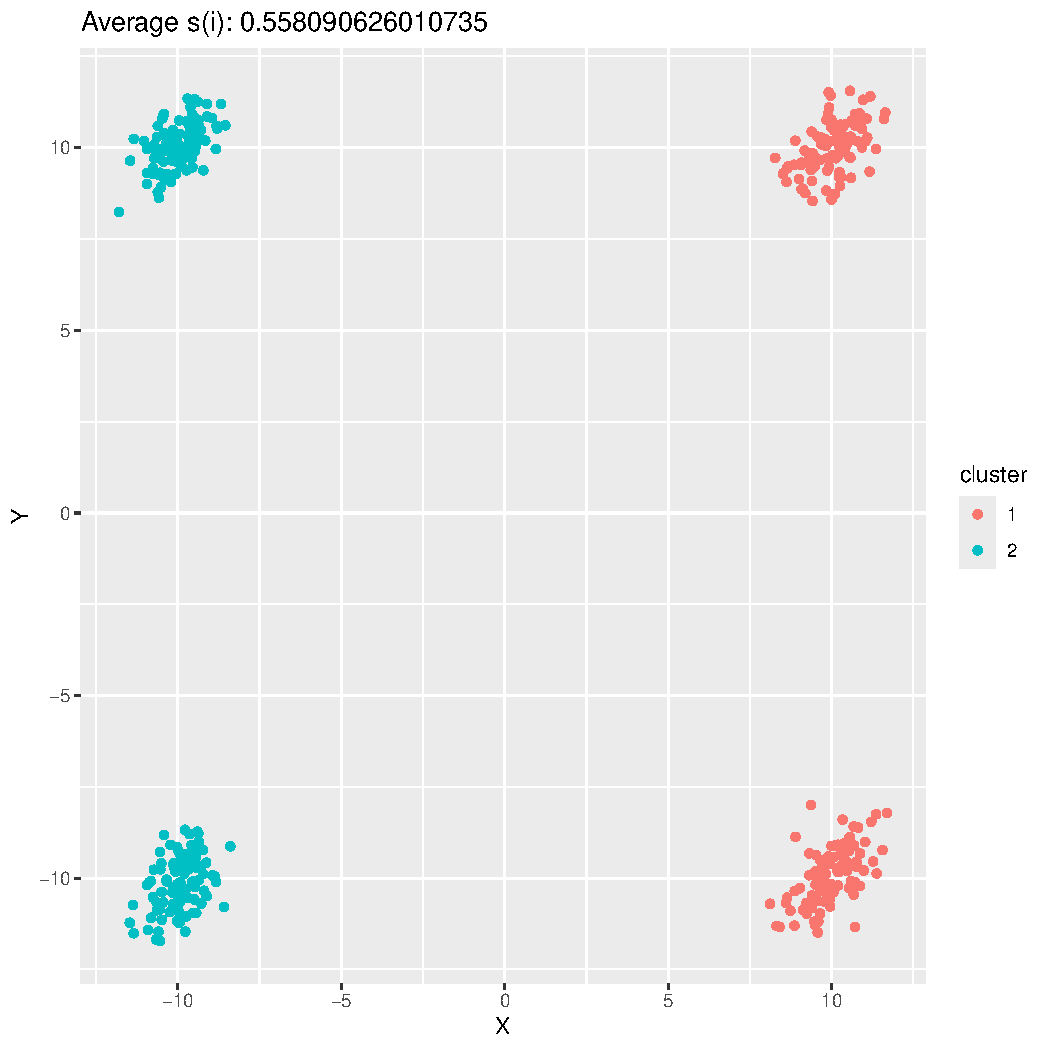
\includegraphics[width = 0.5\textwidth, height = 0.3\textheight]{doc/clusters-2.pdf}
				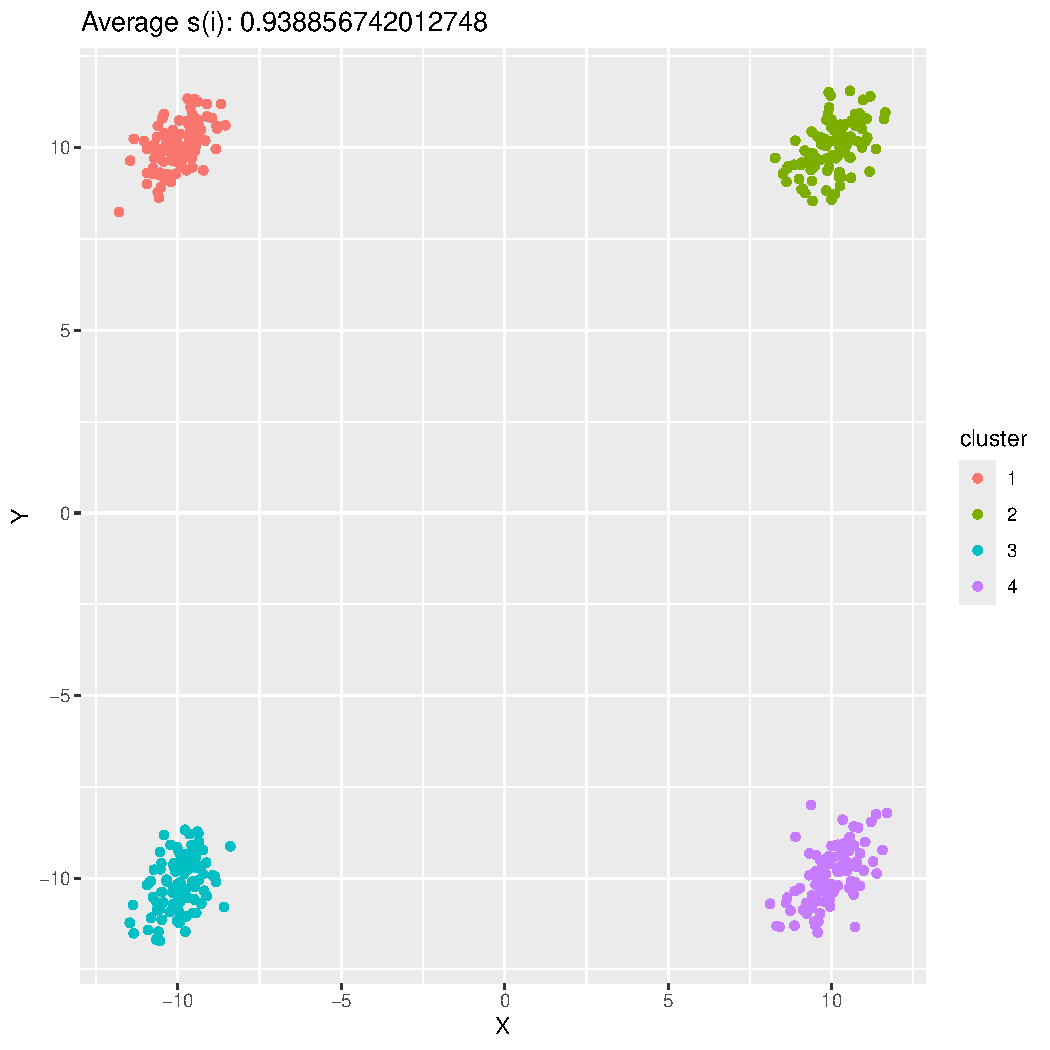
\includegraphics[width = 0.5\textwidth, height = 0.3\textheight]{doc/clusters-4.pdf}
				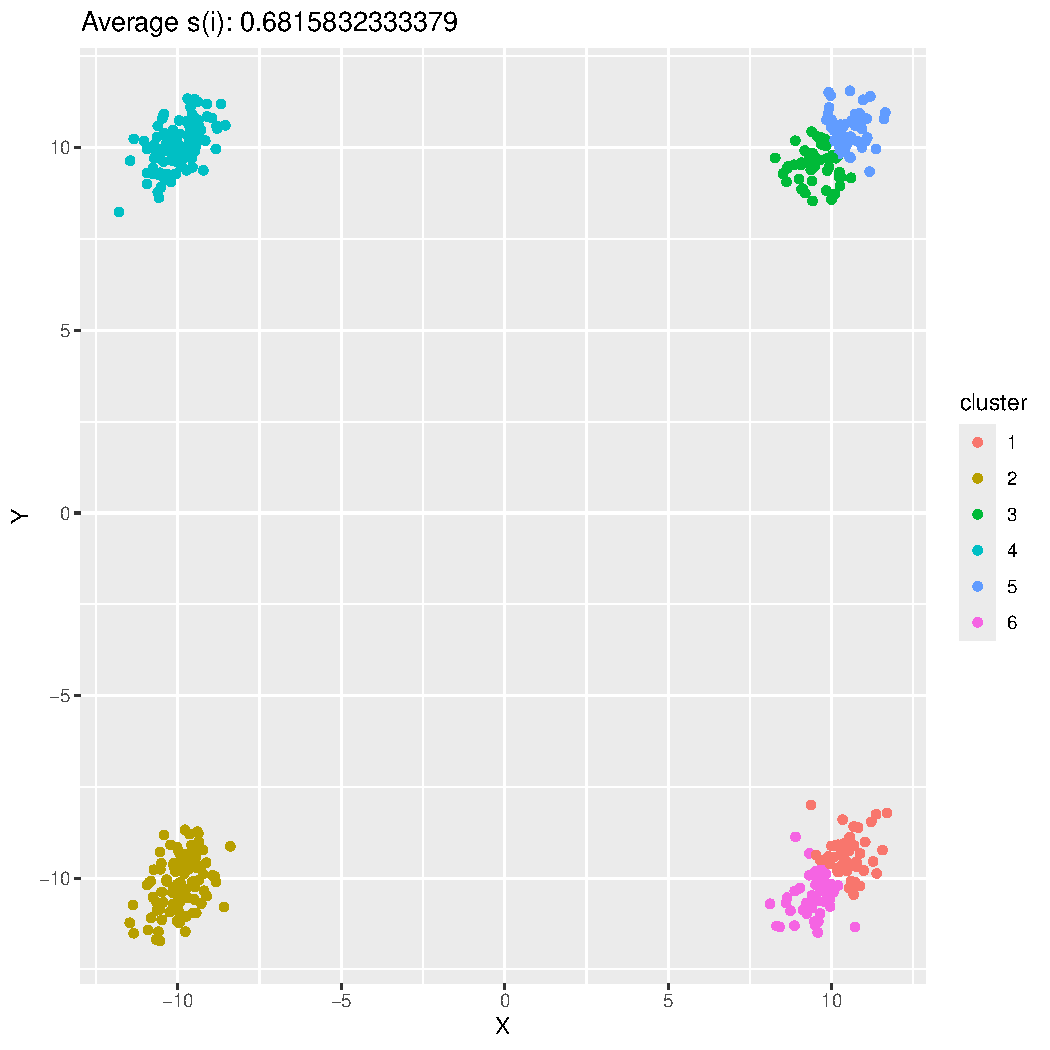
\includegraphics[width = 0.5\textwidth, height = 0.3\textheight]{doc/clusters-6.pdf}
				\caption{Clustering con K-Means usando K = 2, 4, 6 per un dataset
				auto generato in cui la struttura di cluster è ben visibile. }
				\label{fig:k246}
			\end{figure}

			In generale, l'operato di un algoritmo di clustering può
			considerarsi ottimale se il valore si $s(i)$ tende ad essere
			molto alto per tutti gli elementi del dataset. A tale scopo,
			è possibile calcolare la Silhouette media per un certo cluster
			$C$ come la media tutti gli $s(i)$ per ciascun elemento $i$
			che appartiene a $C$. Se tale valore medio è alto, il cluster
			nel suo complesso è ben formato.

			Se si ha invece interesse a sapere qual'è il numero ottimale di
			cluster, è possibile considerare la Silhouette media complessiva
			come la media di tutti gli $s(i)$ per ogni elemento dell'intero
			dataset. L'idea è quella di testare diverse combinazioni di
			iperparametri dell'algoritmo di clustering e scegliere la
			combinazione che restituisce la Silhouette media complessiva più
			grande: tale combinazione sarà quella che restituisce il clustering
			che meglio interpreta il dataset.

			Si noti come un valore della Silhouette media complessiva
			pari a $0$ non significa necessariamente che il clustering
			non sia andato a buon fine. Può infatti anche indicare che
			effettivamente il dataset non ha alcuna struttura di clustering
			naturale, e che quindi l'algoritmo di clustering ha comunque
			fornito un risultato corretto, dato che effettivamente qualsiasi
			risultato vale l'altro.

		\section{Sanity check e matrice binaria}

			Il linguaggio \texttt{R} offre diverse implementazioni del
			calcolo della Silhouette. A differenza di altri linguaggi come
			Python, dove esiste un "consensus" (ufficiale o ufficioso) riguardo
			a quali siano i pacchetti da utilizzare per un determinato scopo,
			su \texttt{R} questo talvolta manca. Pertanto, prima di mettere
			Silhouette sotto analisi, é necessario scegliere un pacchetto fra
			quelli disponibili.

			Ho cercato quante piú implementazioni di Silhouette possibili
			utilizzando il sito \texttt{https://rdrr.io} e scegliendone
			quante più possibili che provenissero dal repository CRAN.
			In particolare, sono stati scelti \texttt{cluster},
			\texttt{drclust}, \texttt{tidyclust} e \texttt{Kira}. Pacchetti
			noti come \texttt{fpc}, che pure implementano Silhouette, li ho
			esclusi a priori perché non aggiornati da tempo.

			Oltre a questi, come controprova ho utilizzato l'implementazione
			della Silhouette presente nel pacchetto \texttt{scikit-learn} per
			\texttt{Python}. Questo è stato fatto attraverso il pacchetto
			\texttt{reticulate}, che permette di chiamare funzioni \texttt{Python}
			all'interno di codice \texttt{R}.

			Per comparare le performance delle diverse implementazioni di
			Silhouette ho eseguito due test, uno chiamato "sanity check" ed
			uno chiamato "matrice binaria". Il codice per la generazione dei
			test è liberamente disponibile. Ho organizzato il codice seguendo
			le linee guida riportate in \cite{10.1371/journal.pcbi.1000424}.
			Ho anche tenuto un lab notebook per tenere traccia dei risultati
			mano mano che venivano generati, facendo riferimento a \cite{10.1371/journal.pcbi.1004385}

			Il test Sanity check prevede di utilizzare due dataset creati
			artificialmente, il primo dove la struttura di cluster è
			estremamente evidente ed il secondo dove la struttura di
			cluster è completamente assente, applicare su questi l'algoritmo
			di clustering K-Means e calcolare sul risultato di quest'ultimo
			la Silhouette media.

			Lo scatter plot dei due dataset è riportato in Figure~\ref{fig:sc}.
			Li ho costruiti utilizzando la funzione \texttt{rnorm}, che genera
			dei punti casuali a partire da una distribuzione normale bivariata.	
			Il primo è stato costruito usando due distribuzioni normali fuse
			insieme, entrambe con una deviazione standard molto bassa, di modo
			che i punti siano concentrati attorno alla media. Il secondo è
			costituito da una sola distribuzione normale centrata in $(0, 0)$
			con una deviazione standard molto ampia, di modo che i punti siano
			molto dispersi.

			\begin{figure}[h]
				\centering
				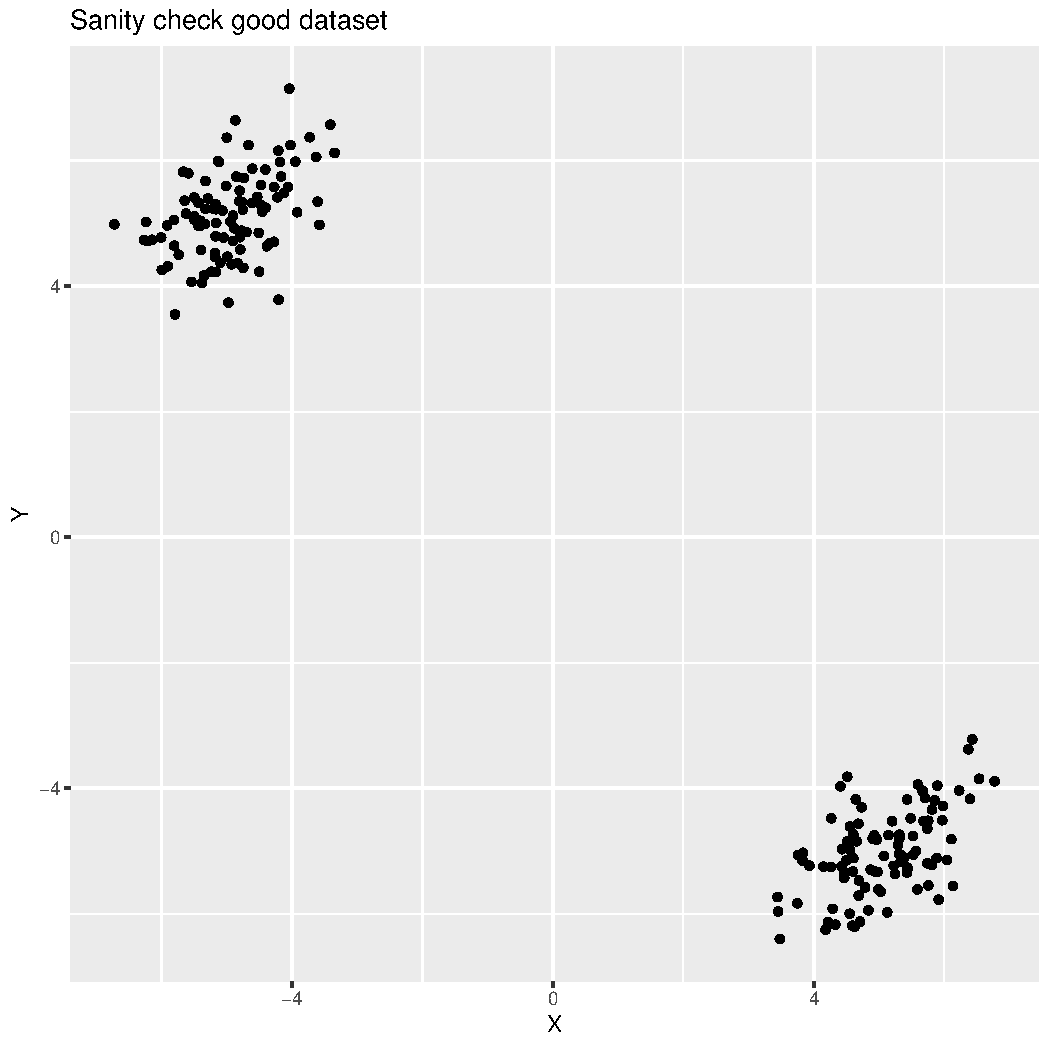
\includegraphics[width = 0.75\textwidth, height = 0.45\textheight]{doc/sc_dataset_good.pdf}
				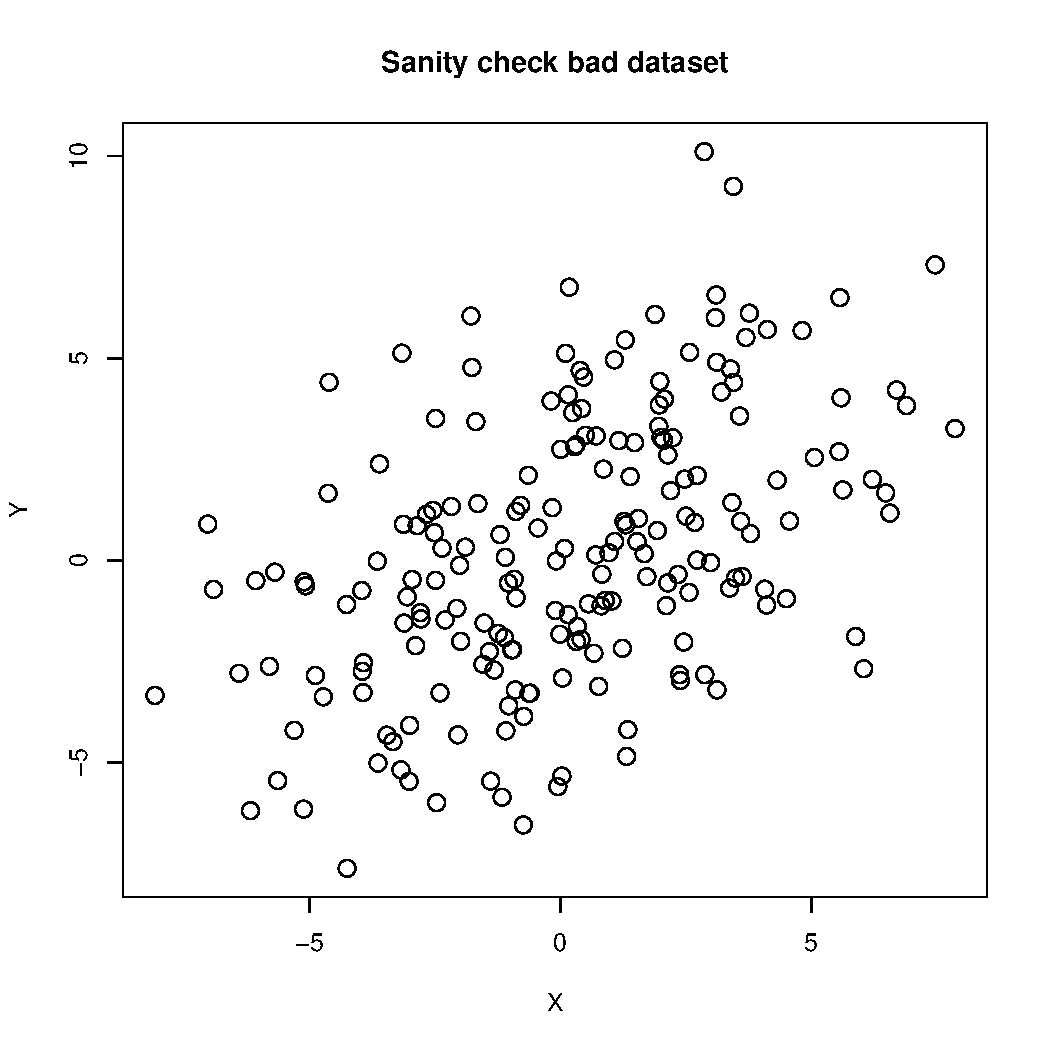
\includegraphics[width = 0.75\textwidth, height = 0.45\textheight]{doc/sc_dataset_bad.pdf}
				\caption{Plot dei dataset per il test sanity check. Il primo
				presenta una struttura di cluster ben definita, mentre nel
				secondo la struttura di cluster è completamente assente.}
				\label{fig:sc}
			\end{figure}

			Il test matrice binaria inizia con una matrice di dimensione
			$2n times n$, costituita per metà da $0$ e per metà da $1$.
			Su tale matrice viene applicato K-Means con iperparametro
			$K = 2$ e si calcola la Silhouette media complessiva del
			risultato. Dopodiché, una qualsiasi delle righe viene sostituita
			con un valore scelto casualmente nell'intervallo $(0, 1)$ e si
			ripete il procedimento. Tale test viene ripetuto esattamente
			$2n$ volte, ogni volta con una riga diversa.

			I $2n$ valori della Silhouette media complessiva così trovati
			sono poi riportati in un plot; l'idea è che tali valori debbano
			essere alti nelle prime istanze del test quando gli $0$ e gli
			$1$ sono ben separati e piano piano perdano si riducano così
			come il dataset perde coesione. Ci si aspetta che i punti sul
			grafico approssimino una distribuzione lineare.

		\section{Algoritmi}

			Gli algoritmi di clustering sono innumerevoli, ed è
			impossibile testarli tutti. In questa tesi ne ho scelti
			quattro: \textbf{K-Means} \cite{1056489} e la sua variante
			\textbf{K-Medians}, \textbf{DBSCAN} \cite{10.5555/3001460.3001507}
			e \textbf{HDBSCAN} \cite{10.1007/978-3-642-37456-2_14}.

			\subsection{Clustering partizionale: K-Means e K-Medians}

				\textbf{K-Means} e \textbf{K-Medians} sono esempi di algoritmi
				di clustering \textbf{partizionale}, ovvero che suddividono
				l'insieme di dati in un certo numero di cluster operando diversi
				"raffinamenti" spostando uno o più elementi da un cluster all'altro
				fino a raggiungere la precisione desiderata. L'algoritmo può essere
				descritto come segue:

				\begin{enumerate}
					\item
						Sia scelga un intero $k$. Tale valore sarà il numero di cluster;
					\item
						Si scelgano $k$ elementi qualsiasi del dataset, detti \textbf{seed}.
						Tali seed fungeranno da \textbf{centroidi} iniziali, ovvero da elementi
						che rappresentano il "baricentro" o il "punto medio" di ciascun cluster;
					\item
						Per ciascun elemento del dataset che non é un centroide, si calcoli
						la distanza fra tale elemento e tutti i centroidi. L'elemento viene
						assegnato alla partizione il cui centroide ha la piú piccola distanza
						da questo;
					\item
						Per ogni cluster se ne ricalcolino i centroidi, operando la media
						aritmetica dei suoi valori;
					\item
						Se é stato raggiunto un criterio di terminazione, l'algoritmo termina.
						Altrimenti, si riprende dal punto 3.
				\end{enumerate}

				Si noti come l'algoritmo non specifichi un criterio di terminazione. Un criterio
				molto semplice consiste nel fissare un $\epsilon$ e valutare di quanto
				si discosta il nuovo valore dei centroidi (calcolato al punto 4) dal
				valore precedente: se questo scostamento é inferiore ad $\epsilon$,
				l'algoritmo termina. Un criterio simile prevede di fissare un $\epsilon$
				e di terminare l'algoritmo se il numero di elementi che vengono assegnati
				ad un cluster diverso alla fine della corrente iterazione é inferiore ad
				$\epsilon$.

				\begin{figure}[H]
					\centering
					\includesvg{images/K-Means-Example}
					\caption{Applicazione dell'algoritmo K-Means ad un ipotetico dataset;
					i tre colori indicano i tre cluster individuati dall'algoritmo (By I,
					Weston.pace, CC BY-SA 3.0, https://commons.wikimedia.org/w/index.php?curid=2463085).}
					\label{fig:k-means-example}
				\end{figure}

				L'algoritmo K-Medians è una variante di K-Means che usa le mediane dei
				cluster come centroidi anzichè le loro medie. Per tal motivo, mentre
				K-Means può utilizzare sostanzialmente qualsiasi funzione di distanza,
				K-Medians utilizza sempre la distanza di Manhattan.

				Sebbene K-Means e K-Medians siano efficienti (se il numero di
				iterazioni è piccolo, il tempo di esecuzione è quasi-lineare) e
				anche estremamente semplici, tanto da comparire come subroutine
				in algoritmi più complessi, presentano dei problemi. Ad esempio,
				dato che ogni elemento ha lo stesso peso nel computo dei centroidi,
				anche un solo elemento che abbia valori anomali può destabilizzare
				completamente il risultato finale. Inoltre, il parametro $k$ che
				determina il numero di cluster potrebbe non avere alcuna relazione
				con l'effettivo numero di cluster (se esistono) nell'insieme di
				dati, e quindi un valore scorretto di $k$ porta a risultati che
				non rispecchiano per nulla la vera struttura di cluster. Infine,
				il raggruppamento di piú elementi sulla base di una distanza genera
				dei cluster di forma ellittica, ma non tutti i dataset hanno una
				struttura di cluster con questa forma.

			\subsection{Clustering per densità: DBSCAN}

				\textbf{DBSCAN} è un esempio di algoritmo di clustering \textbf{per
				densità}, ovvero che costruisce i cluster a partire da come gli
				elementi di un dataset sono aggregati. In questo senso, i cluster
				figurano come regioni di spazio densamente popolate, di forma del
				tutto arbitraria, separate da spazio poco popolato.

				DBSCAN prevede che vengano innanzitutto scelti due valori, un intero
				chiamato MinPts ed un numero reale positivo $\epsilon$. A partire da
				questi, per ogni elemento $p$ del dataset è possibile definire un
				insieme $N_{\epsilon}(p)$, chiamato $\epsilon$\textbf{-vicinato}
				($\epsilon$\textbf{-neighbourhood}). Tale insieme contiene tutti i
				punti $q$ che hanno distanza da $p$ inferiore a $\epsilon$:

				\begin{equation*}
					N_{\epsilon} (p) = \{q | d(p, q) \leq \epsilon\}
				\end{equation*}

				Ogni elemento $p$ del dataset viene classificato sulla base del numero
				di elementi di $N_{\epsilon}(p)$:

				\begin{itemize}
					\item
					Se $N_{\epsilon}(p)$ ha almeno MinPts elementi, si dice che $p$ è un
					\textbf{core point};
					\item
					Se $N_{\epsilon}(p)$ ha meno di MinPts elementi ma $p$ si trova
					nell'$\epsilon$-vicinato di un altro elemento, allora si dice che
					$p$ è un \textbf{border point};
					\item
					Se un elemento non non é né un core point né un border
					point, é detto \textbf{noise point}.
				\end{itemize}

				Si dice che un elemento $q$ é \textbf{direttamente raggiungibile}
				da $p$ se $p$ é un core point e $q$ si trova nell'$\epsilon$-vicinato
				di $p$. Se un elemento $r$ é direttamente raggiungibile da $q$ e $q$
				é direttamente raggiungibile da un elemento $p$, allora si dice che
				$r$ é \textbf{indirettamente raggiungibile} da $p$ (si noti come
				la raggiungibilità non sia una proprietà necessariamente simmetrica).

				\begin{figure}[H]
					\centering
					\includesvg[width = 0.5\textwidth]{images/DBSCAN-Illustration.svg}
					\caption{Ipotetica classificazione di alcuni elementi, usando
					MinPts = 4. Gli elementi in rosso sono dei core point, perchè
					hanno 4 o più elementi nel loro $\epsilon$-vicinato. Gli elementi
					in giallo sono invece border point, perchè hanno meno di 4 elementi
					nel loro $\epsilon$-vicinato ma sono nell'$\epsilon$-vicinato di
					almeno un core point. Infine, gli elementi in blu sono dei
					noise point, perchè oltre ad avere meno di 4 elementi nel loro
					$\epsilon$-vicinato non sono nell'$epsilon$-vicinato di alcun
					core point (By Chire - Own work, CC BY-SA 3.0,
					https://commons.wikimedia.org/w/index.php?curid=17045963).}
					\label{fig:dbscan-illustration}
				\end{figure}

				Quando DBSCAN viene invocato viene inizializzato un cluster
				$C$, dopodiché viene costruito l'$\epsilon$-vicinato di ogni
				elemento $p$ che non sia stato ancora ispezionato. Se tale
				insieme ha meno di MinPts elementi, allora $p$ é certamente
				un noise point: questo perché é troppo isolato per poter
				essere un core point e, non essendo ancora stato ispezionato,
				non puó trovarsi nell'$\epsilon$-vicinato di nessun altro punto.

				Se invece l'$\epsilon$-vicinato di $p$ ha almeno MinPts
				elementi, allora tale elemento é certamente un core point.
				Viene allora costruito un cluster $C$ nel quale $p$ viene
				inserito, dopodiché vengono osservati tutti gli elementi
				$q$ che si trovano nell'$\epsilon$-vicinato di $p$.
				Se $q$ non é mai stato ispezionato, si osserva
				l'$\epsilon$-vicinato di $q$ a sua volta: se questo
				contiene piú elementi dell'$\epsilon$-vicinato di $p$,
				allora $N_{\epsilon}(q)$ e $N_{\epsilon}(p)$ vengono
				uniti in un insieme unico, perché gli elementi
				dell'$\epsilon$-vicinato di $q$ sono indirettamente
				raggiungibili a partire da $p$. Se $q$ non appartiene
				ad alcun cluster, allora viene aggiunto al cluster in esame.

				\begin{figure}[H]
					\centering
					\includesvg[width = 0.5\textwidth]{images/DBSCAN-density-data.svg}
					\caption{Risultato dell'applicazione dell'algoritmo DBSCAN su un
					ipotetico dataset. Le aree in blu e in verde rappresentano i due
					cluster, mentre i punti in grigio sono i noise point (By Chire -
					Own work, CC BY-SA 3.0, https://commons.wikimedia.org/w/index.php?curid=17085332)}
					\label{fig:dbscan-density-data}
				\end{figure}

				Si osservi come la scelta di $\epsilon$ e MinPts influisca di molto
				sul risultato finale. Infatti, scegliendo un valore di $\epsilon$ o
				di MinPts troppo piccolo, quasi tutti gli elementi verranno classificati
				come noise point, e quindi quasi tutti scartati. D'altro canto, un valore
				di $\epsilon$ o di MinPts troppo grande potrebbe indurre un clustering
				dove quasi tutti i punti sono inclusi nello stesso cluster.

				A differenza di K-Means e K-Medians, che costruiscono sempre cluster
				di forma ellissoidale, DBSCAN costruisce cluster di qualsiasi forma.
				Questo è sia un aspetto positivo, perchè in questo modo è possibile
				catturare strutture di cluster molto più variegate, sia negativo,
				perchè la densità di un'area non sottende necessariamente alla
				presenza di un cluster, e non tutte le aree dense lo sono allo
				stesso modo. Occorre però evidenziare come, nonostante sia leggermente
				inferiore a K-Means e K-Medians in termini di tempo di esecuzione
				($O n \log(n)$, con $n$ numero di elementi del dataset), le sue
				prestazioni sono state empiricamente dimostrate come molto competitive.

			\subsection{Clustering gerarchico: HDBSCAN}

				\textbf{HDBSCAN} é un esempio di algoritmo di clustering
				\textbf{gerarchico}, ovvero che costruisce i cluster formando
				una struttura ad albero \footnote{In realtá, HDBSCAN é un
				algoritmo ibrido fra il paradigma per densitá ed il paradigma
				gerarchico. Un esempio semplice di algoritmo di clustering
				``puramente'' gerarchico é \textbf{UPGMA} \cite{Sokal1958ASM}.}

	\chapter{Risultati}

		\section{Risultati dei test}

			I risultati per il test sanity check sono riportati di seguito.
			Il test sanity check non é stato particolarmente conclusivo,
			perché tutti e cinque i pacchetti hanno fornito valori molto
			simili (circa $0.9$ per il primo dataset e circa $0.4$ per il
			secondo). Questo é un risultato atteso, perché il test era
			appositamente costruito per escludere pacchetti problematici.

			\begin{figure}[h]
				\begin{boxedminipage}{0.5\textwidth}
					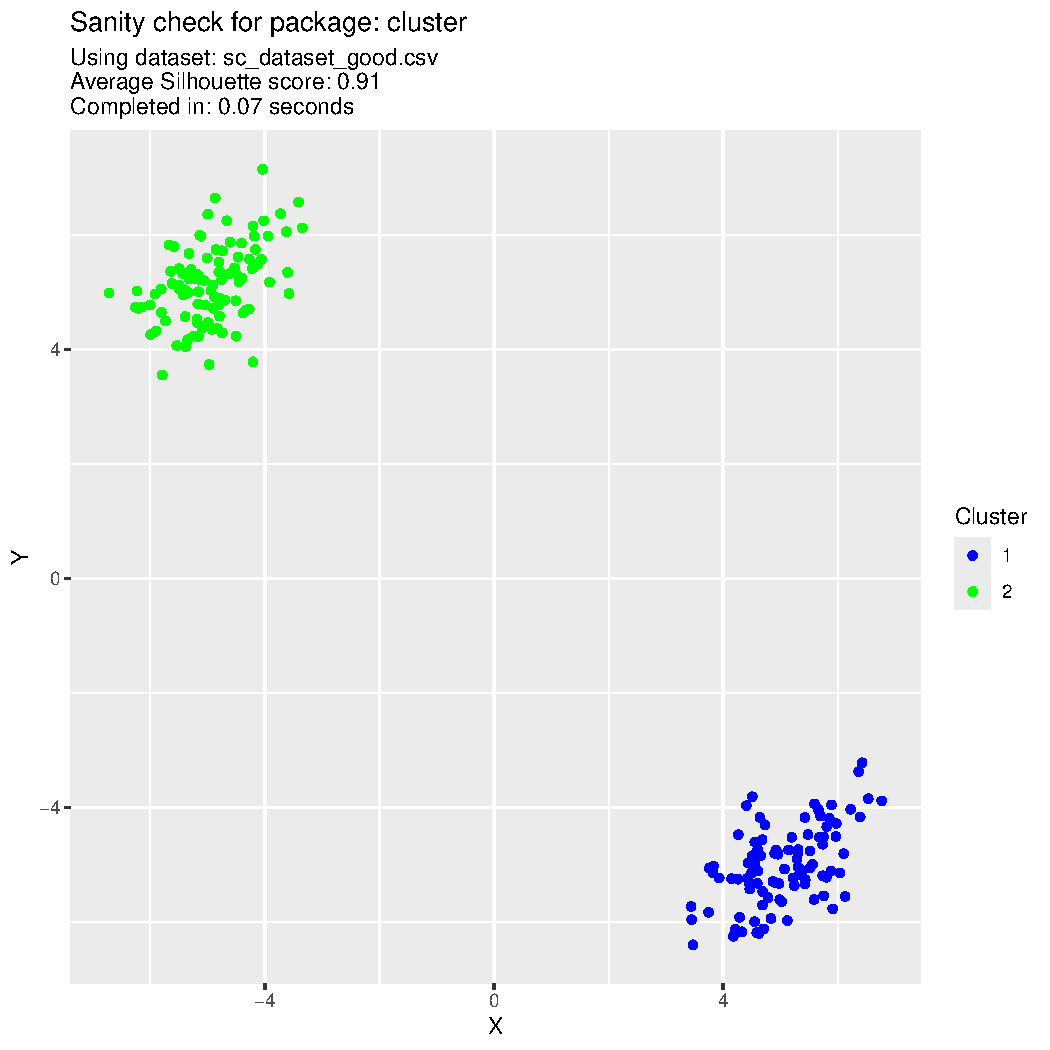
\includegraphics[width = \textwidth, page = 1]{results/results_CLUSTER.pdf}
				\end{boxedminipage}
				\begin{boxedminipage}{0.5\textwidth}
					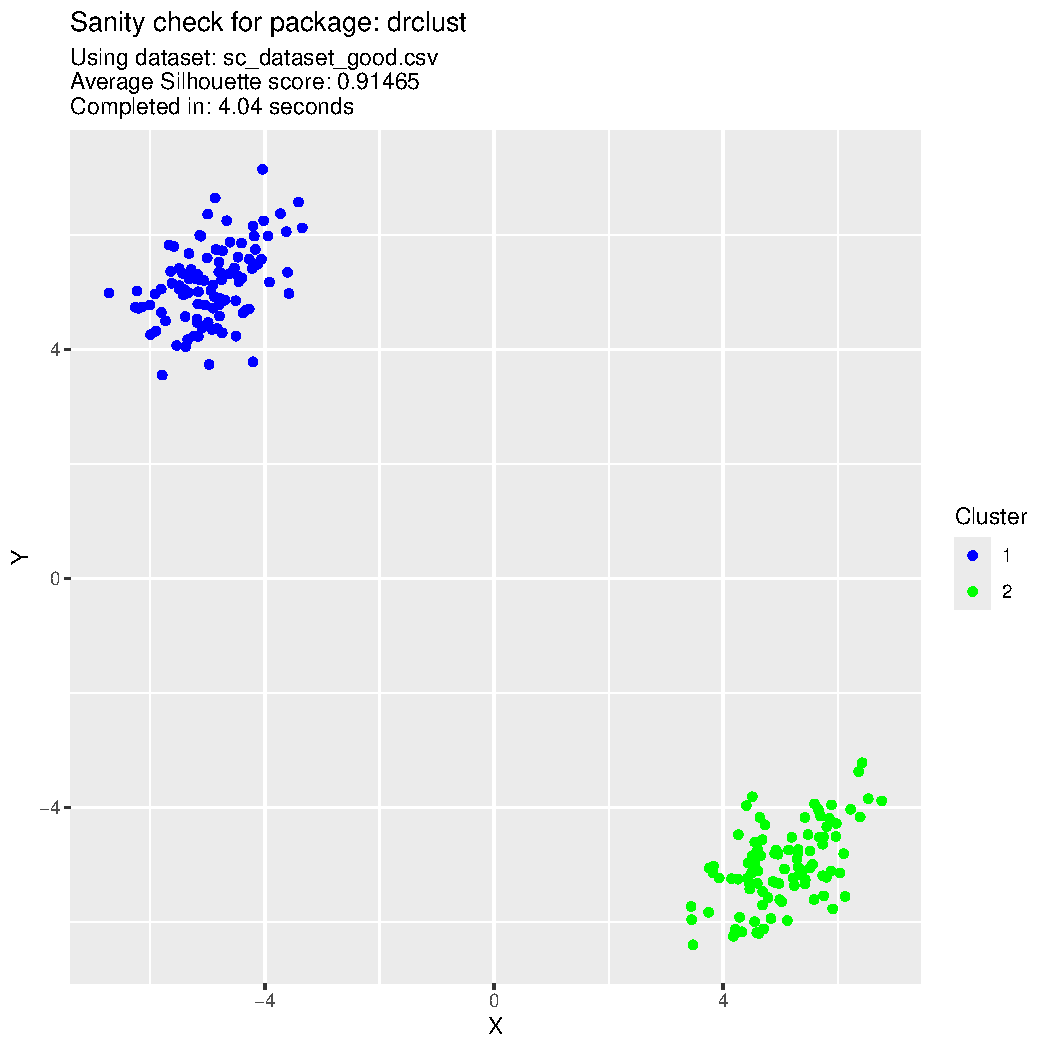
\includegraphics[width = \textwidth, page = 1]{results/results_DRCLUST.pdf}
				\end{boxedminipage}
				\begin{boxedminipage}{0.5\textwidth}
					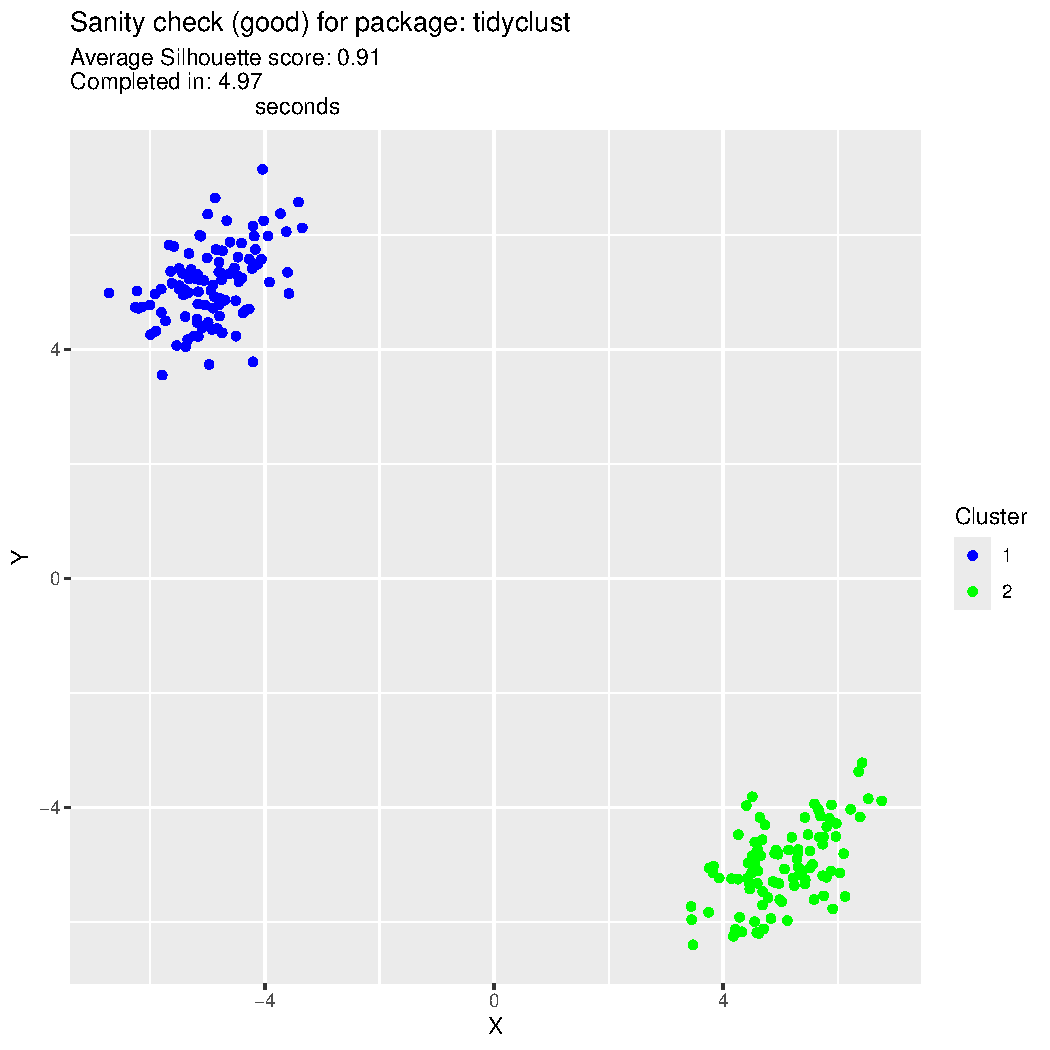
\includegraphics[width = \textwidth, page = 1]{results/results_TIDYCLUST.pdf}
				\end{boxedminipage}
				\begin{boxedminipage}{0.5\textwidth}
					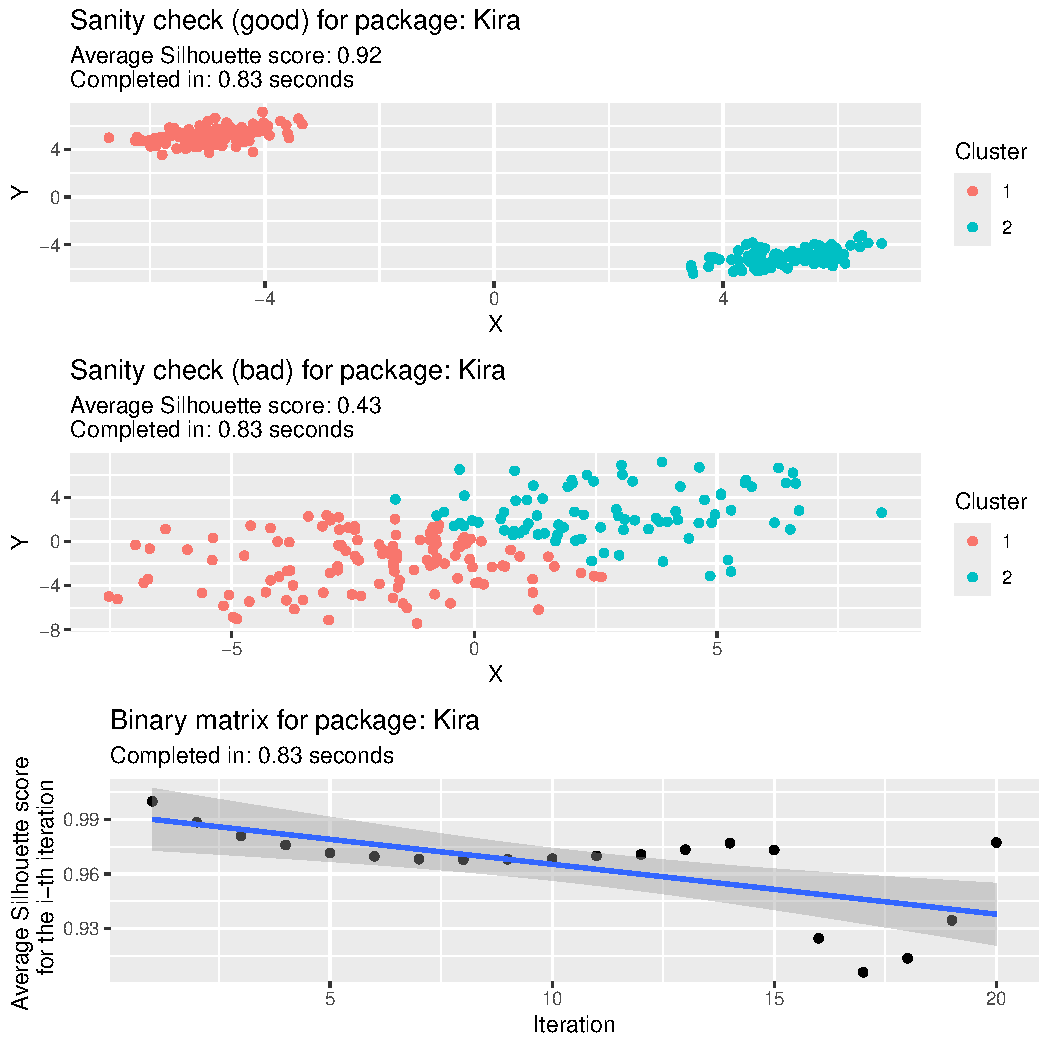
\includegraphics[width = \textwidth, page = 1]{results/results_KIRA.pdf}
				\end{boxedminipage}
				\caption{Plot dei test sanity check usando il dataset con struttura di cluster
				ben visibile.}
				\label{fig:good}
			\end{figure}

			\begin{figure}[h]
				\begin{boxedminipage}{0.5\textwidth}
					\includegraphics[width = \textwidth, page = 2]{results/results_CLUSTER.pdf}
				\end{boxedminipage}
				\begin{boxedminipage}{0.5\textwidth}
					\includegraphics[width = \textwidth, page = 2]{results/results_DRCLUST.pdf}
				\end{boxedminipage}
				\begin{boxedminipage}{0.5\textwidth}
					\includegraphics[width = \textwidth, page = 2]{results/results_TIDYCLUST.pdf}
				\end{boxedminipage}
				\begin{boxedminipage}{0.5\textwidth}
					\includegraphics[width = \textwidth, page = 2]{results/results_KIRA.pdf}
				\end{boxedminipage}
				\caption{Plot dei test sanity check usando il dataset con struttura di cluster
				assente.}
				\label{fig:bad}
			\end{figure}

			\begin{figure}[h]
				\centering
				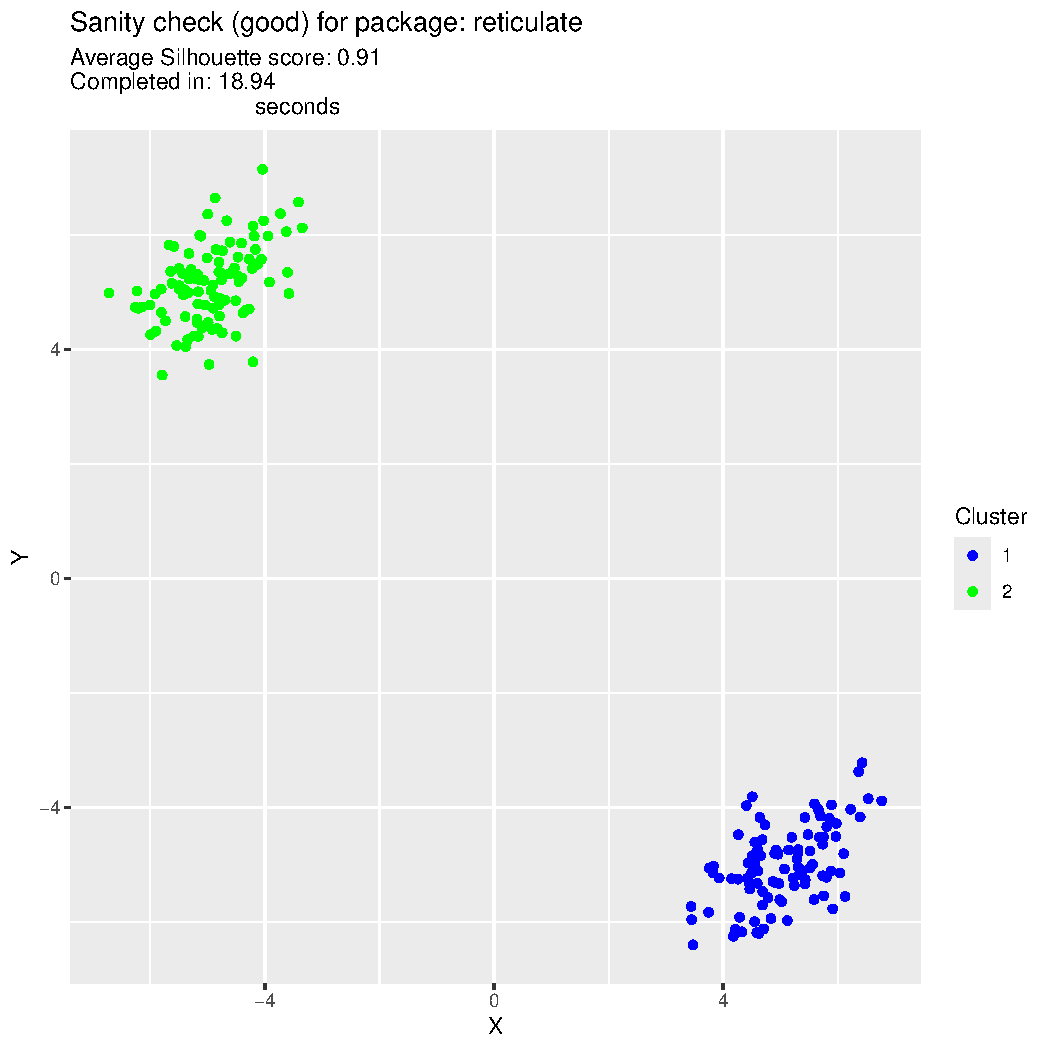
\includegraphics[width = 0.75\textwidth, height = 0.45\textheight, page = 1]{results/results_RETICULATE.pdf}
				\includegraphics[width = 0.75\textwidth, height = 0.45\textheight, page = 2]{results/results_RETICULATE.pdf}
				\caption{Plot del test sanity check usando \texttt{scikit-learn} attraverso
				\texttt{reticulate}.}
				\label{fig:reticulate}
			\end{figure}

			I risultati per il test matrice binaria sono riportati
			di seguito. Il test é stato piú informativo del precedente,
			perché i valori restituiti avevano delle differenze
			evidenziabili. In particolare, \texttt{Kira} é stato il
			pacchetto con le performance peggiori, perché i valori
			della Silhouette media complessiva sono rimasti pressoché
			identici. I pacchetti \texttt{cluster}, \texttt{drclust}
			e \texttt{tidyclust} hanno invece avuto risultati molto
			simili. In particolare, \texttt{cluster} e \texttt{tidyclust}
			hanno avuto risultati perfettamente identici, segno che
			probabilmente l'uno usa l'altro come subroutine.

			\begin{figure}[h]
				\begin{boxedminipage}{0.5\textwidth}
					\includegraphics[width = \textwidth, page = 3]{results/results_CLUSTER.pdf}
				\end{boxedminipage}
				\begin{boxedminipage}{0.5\textwidth}
					\includegraphics[width = \textwidth, page = 3]{results/results_DRCLUST.pdf}
				\end{boxedminipage}
				\begin{boxedminipage}{0.5\textwidth}
					\includegraphics[width = \textwidth, page = 3]{results/results_TIDYCLUST.pdf}
				\end{boxedminipage}
				\begin{boxedminipage}{0.5\textwidth}
					\includegraphics[width = \textwidth, page = 3]{results/results_KIRA.pdf}
				\end{boxedminipage}
				\caption{Plot dei test matrice binaria.}
				\label{fig:bm}
			\end{figure}

			\begin{figure}[h]
				\includegraphics[width = \textwidth, page = 3]{results/results_RETICULATE.pdf}
				\caption{Plot del test matrice binaria per il pacchetto
				\texttt{scikit-learn} (attraverso \texttt{reticulate})}
				\label{fig:reticulatebm}
			\end{figure}

		\section{Risultati delle applicazioni su EHR}

			Per K-Means, è stato testato un numero di cluster compreso fra $2$ e
			$6$, mentre per K-Medians fra $2$ e $10$.

			Per DBSCAN e HDBSCAN, MinPts è stato scelto nel range dal numero delle
			dimensioni del dataset al doppio più uno delle dimensioni del dataset.

			Per DBSCAN, $\epsilon$ è stato scelto partizionando la distanza massima
			in parti uguali.

			\begin{figure}[h]
				\centering
				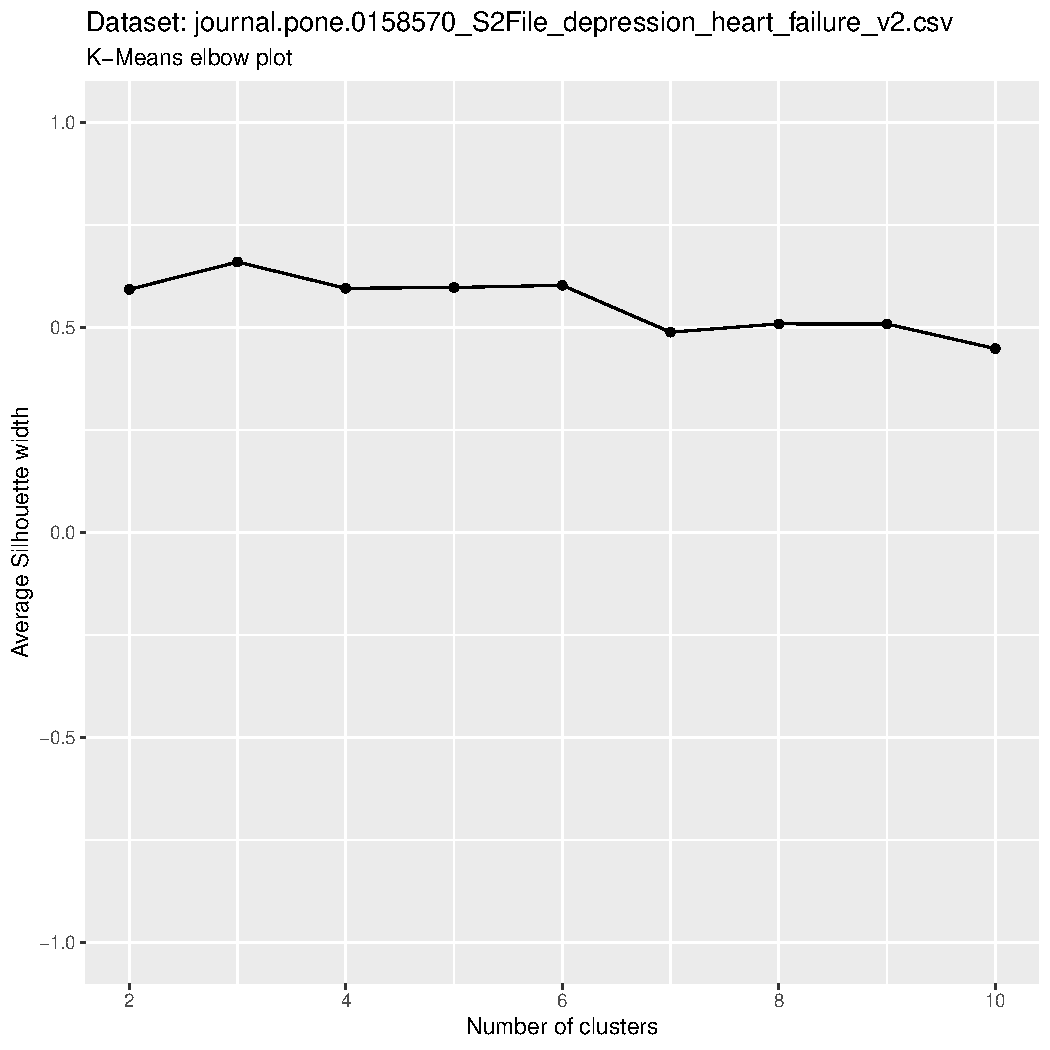
\includegraphics[width = 0.75\textwidth, height = 0.45\textheight, page = 1]{
					results/results_journal.pone.0158570_S2File_depression_heart_failure_v2.csv.pdf
				}
				\includegraphics[width = 0.75\textwidth, height = 0.45\textheight, page = 2]{
					results/results_journal.pone.0158570_S2File_depression_heart_failure_v2.csv.pdf
				}
				\caption{Risultati dell'algoritmo K-Means per il dataset
				\texttt{results\_journal.pone.0158570\_S2File\_depression\_heart\_failure\_v2.csv}}
				\label{fig:kmeans1}
			\end{figure}

			\begin{figure}[h]
				\centering
				\includegraphics[width = 0.75\textwidth, height = 0.45\textheight, page = 3]{
					results/results_journal.pone.0158570_S2File_depression_heart_failure_v2.csv.pdf
				}
				\includegraphics[width = 0.75\textwidth, height = 0.45\textheight, page = 4]{
					results/results_journal.pone.0158570_S2File_depression_heart_failure_v2.csv.pdf
				}
				\caption{Risultati dell'algoritmo K-Medians per il dataset
				\texttt{results\_journal.pone.0158570\_S2File\_depression\_heart\_failure\_v2.csv}}
				\label{fig:kmedians1}
			\end{figure}

			\begin{figure}[h]
				\centering
				\includegraphics[width = 0.75\textwidth, height = 0.45\textheight, page = 5]{
					results/results_journal.pone.0158570_S2File_depression_heart_failure_v2.csv.pdf
				}
				\includegraphics[width = 0.75\textwidth, height = 0.45\textheight, page = 6]{
					results/results_journal.pone.0158570_S2File_depression_heart_failure_v2.csv.pdf
				}
				\caption{Risultati dell'algoritmo DBSCAN per il dataset
				\texttt{results\_journal.pone.0158570\_S2File\_depression\_heart\_failure\_v2.csv}}
				\label{fig:dbscan1}
			\end{figure}

			\begin{figure}[h]
				\centering
				\includegraphics[width = 0.75\textwidth, height = 0.45\textheight, page = 7]{
					results/results_journal.pone.0158570_S2File_depression_heart_failure_v2.csv.pdf
				}
				\includegraphics[width = 0.75\textwidth, height = 0.45\textheight, page = 8]{
					results/results_journal.pone.0158570_S2File_depression_heart_failure_v2.csv.pdf
				}
				\caption{Risultati dell'algoritmo HDBSCAN per il dataset
				\texttt{results\_journal.pone.0158570\_S2File\_depression\_heart\_failure\_v2.csv}}
				\label{fig:hdbscan1}
			\end{figure}

			\begin{figure}[h]
				\centering
				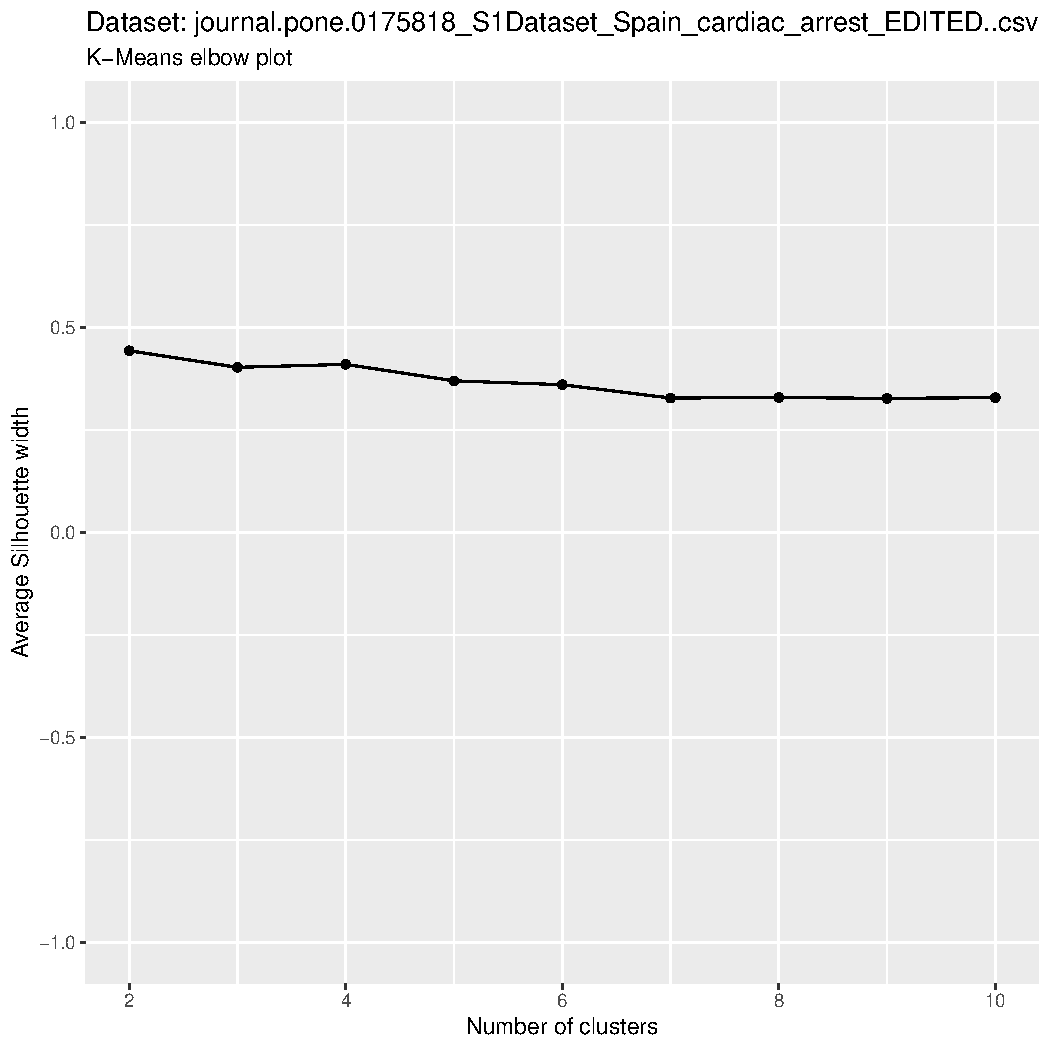
\includegraphics[width = 0.75\textwidth, height = 0.45\textheight, page = 1]{
					results/results_journal.pone.0175818_S1Dataset_Spain_cardiac_arrest_EDITED..csv.pdf
				}
				\includegraphics[width = 0.75\textwidth, height = 0.45\textheight, page = 2]{
					results/results_journal.pone.0175818_S1Dataset_Spain_cardiac_arrest_EDITED..csv.pdf
				}
				\caption{Risultati dell'algoritmo K-Means per il dataset
				\texttt{results\_journal.pone.0175818\_S1Dataset\_Spain\_cardiac\_arrest\_EDITED..csv}}
				\label{fig:kmeans2}
			\end{figure}

			\begin{figure}[h]
				\centering
				\includegraphics[width = 0.75\textwidth, height = 0.45\textheight, page = 3]{
					results/results_journal.pone.0175818_S1Dataset_Spain_cardiac_arrest_EDITED..csv.pdf
				}
				\includegraphics[width = 0.75\textwidth, height = 0.45\textheight, page = 4]{
					results/results_journal.pone.0175818_S1Dataset_Spain_cardiac_arrest_EDITED..csv.pdf
				}
				\caption{Risultati dell'algoritmo K-Medians per il dataset
				\texttt{results\_journal.pone.0175818\_S1Dataset\_Spain\_cardiac\_arrest\_EDITED..csv}}
				\label{fig:kmedians2}
			\end{figure}

			\begin{figure}[h]
				\centering
				\includegraphics[width = 0.75\textwidth, height = 0.45\textheight, page = 5]{
					results/results_journal.pone.0175818_S1Dataset_Spain_cardiac_arrest_EDITED..csv.pdf
				}
				\includegraphics[width = 0.75\textwidth, height = 0.45\textheight, page = 6]{
					results/results_journal.pone.0175818_S1Dataset_Spain_cardiac_arrest_EDITED..csv.pdf
				}
				\caption{Risultati dell'algoritmo DBSCAN per il dataset
				\texttt{results\_journal.pone.0175818\_S1Dataset\_Spain\_cardiac\_arrest\_EDITED..csv}}
				\label{fig:dbscan2}
			\end{figure}

			\begin{figure}[h]
				\centering
				\includegraphics[width = 0.75\textwidth, height = 0.45\textheight, page = 7]{
					results/results_journal.pone.0175818_S1Dataset_Spain_cardiac_arrest_EDITED..csv.pdf
				}
				\includegraphics[width = 0.75\textwidth, height = 0.45\textheight, page = 8]{
					results/results_journal.pone.0175818_S1Dataset_Spain_cardiac_arrest_EDITED..csv.pdf
				}
				\caption{Risultati dell'algoritmo HDBSCAN per il dataset
				\texttt{results\_journal.pone.0175818\_S1Dataset\_Spain\_cardiac\_arrest\_EDITED..csv}}
				\label{fig:hdbscan2}
			\end{figure}

			\begin{figure}[h]
				\centering
				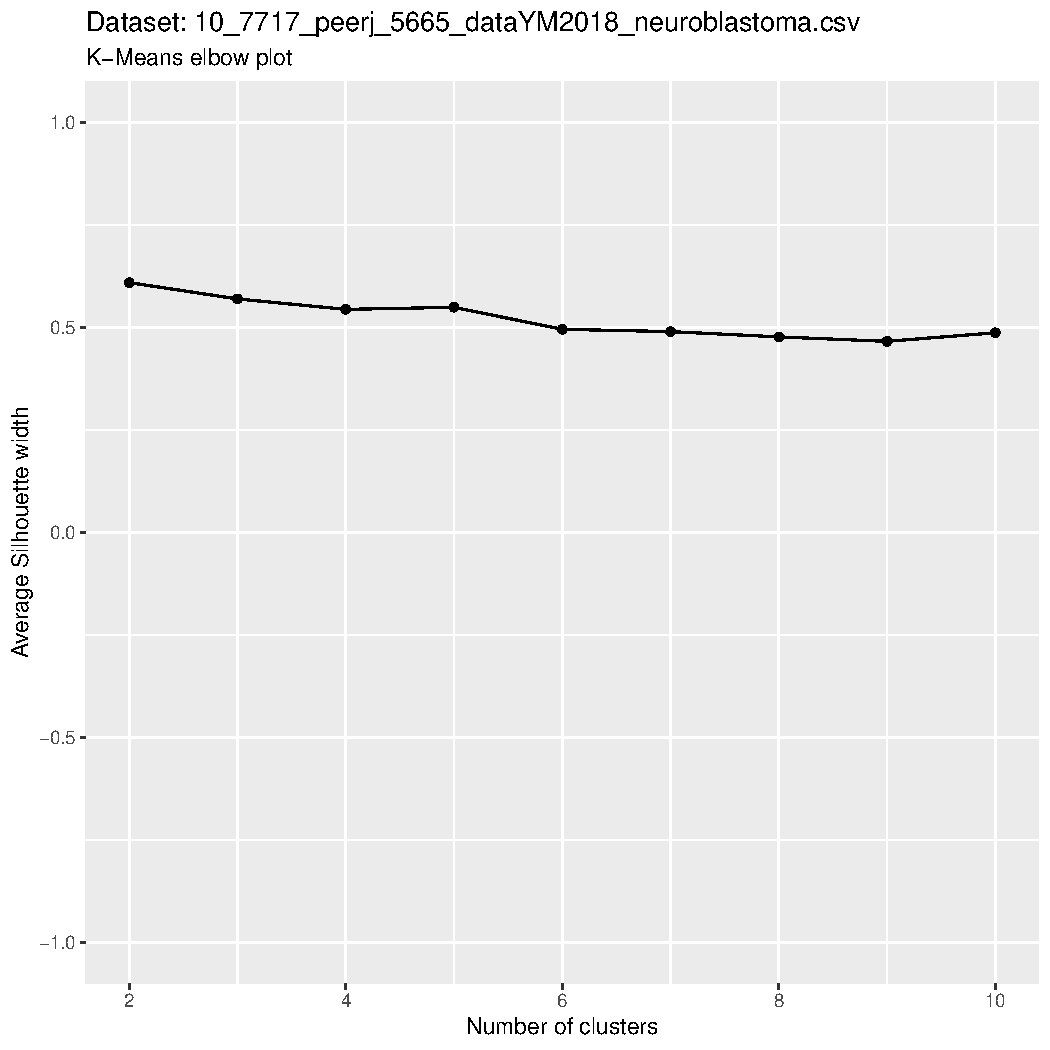
\includegraphics[width = 0.75\textwidth, height = 0.45\textheight, page = 1]{
					results/results_10_7717_peerj_5665_dataYM2018_neuroblastoma.csv.pdf
				}
				\includegraphics[width = 0.75\textwidth, height = 0.45\textheight, page = 2]{
					results/results_10_7717_peerj_5665_dataYM2018_neuroblastoma.csv.pdf
				}
				\caption{Risultati dell'algoritmo K-Means per il dataset
				\texttt{results\_10\_7717\_peerj\_5665\_dataYM2018\_neuroblastoma.csv}}
				\label{fig:kmeans3}
			\end{figure}

			\begin{figure}[h]
				\centering
				\includegraphics[width = 0.75\textwidth, height = 0.45\textheight, page = 3]{
					results/results_10_7717_peerj_5665_dataYM2018_neuroblastoma.csv.pdf
				}
				\includegraphics[width = 0.75\textwidth, height = 0.45\textheight, page = 4]{
					results/results_10_7717_peerj_5665_dataYM2018_neuroblastoma.csv.pdf
				}
				\caption{Risultati dell'algoritmo K-Medians per il dataset
				\texttt{results\_10\_7717\_peerj\_5665\_dataYM2018\_neuroblastoma.csv}}
				\label{fig:kmedians3}
			\end{figure}

			\begin{figure}[h]
				\centering
				\includegraphics[width = 0.75\textwidth, height = 0.45\textheight, page = 5]{
					results/results_10_7717_peerj_5665_dataYM2018_neuroblastoma.csv.pdf
				}
				\includegraphics[width = 0.75\textwidth, height = 0.45\textheight, page = 6]{
					results/results_10_7717_peerj_5665_dataYM2018_neuroblastoma.csv.pdf
				}
				\caption{Risultati dell'algoritmo DBSCAN per il dataset
				\texttt{results\_10\_7717\_peerj\_5665\_dataYM2018\_neuroblastoma.csv}}
				\label{fig:dbscan3}
			\end{figure}

			\begin{figure}[h]
				\centering
				\includegraphics[width = 0.75\textwidth, height = 0.45\textheight, page = 7]{
					results/results_10_7717_peerj_5665_dataYM2018_neuroblastoma.csv.pdf
				}
				\includegraphics[width = 0.75\textwidth, height = 0.45\textheight, page = 8]{
					results/results_10_7717_peerj_5665_dataYM2018_neuroblastoma.csv.pdf
				}
				\caption{Risultati dell'algoritmo HDBSCAN per il dataset
				\texttt{results\_10\_7717\_peerj\_5665\_dataYM2018\_neuroblastoma.csv}}
				\label{fig:hdbscan3}
			\end{figure}

			\begin{figure}[h]
				\centering
				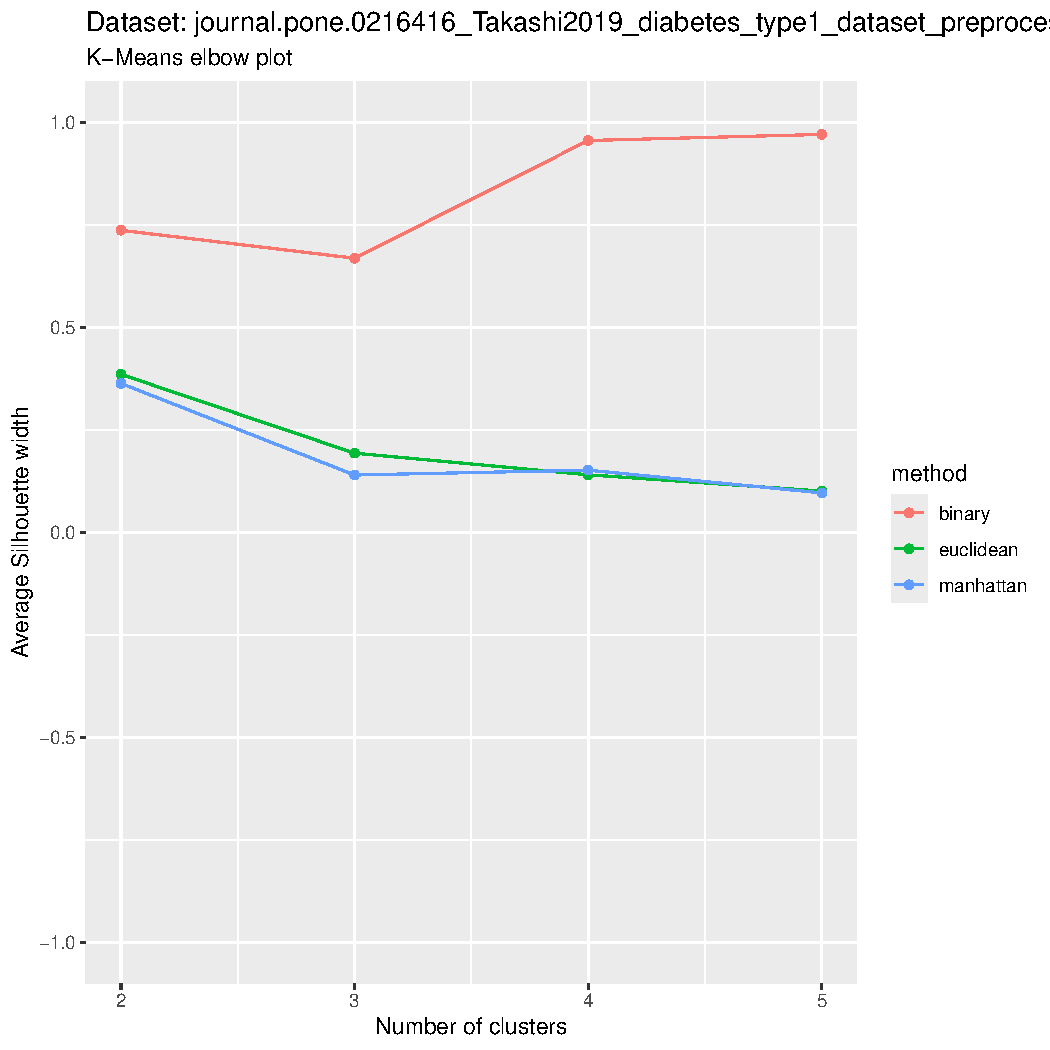
\includegraphics[width = 0.75\textwidth, height = 0.45\textheight, page = 1]{
					results/results_journal.pone.0216416_Takashi2019_diabetes_type1_dataset_preprocessed.csv.pdf
				}
				\includegraphics[width = 0.75\textwidth, height = 0.45\textheight, page = 2]{
					results/results_journal.pone.0216416_Takashi2019_diabetes_type1_dataset_preprocessed.csv.pdf
				}
				\caption{Risultati dell'algoritmo K-Means per il dataset
				\texttt{results\_journal.pone.0216416\_Takashi2019\_diabetes\_type1\_dataset\_preprocessed.csv}}
				\label{fig:kmeans4}
			\end{figure}

			\begin{figure}[h]
				\centering
				\includegraphics[width = 0.75\textwidth, height = 0.45\textheight, page = 3]{
					results/results_journal.pone.0216416_Takashi2019_diabetes_type1_dataset_preprocessed.csv.pdf
				}
				\includegraphics[width = 0.75\textwidth, height = 0.45\textheight, page = 4]{
					results/results_journal.pone.0216416_Takashi2019_diabetes_type1_dataset_preprocessed.csv.pdf
				}
				\caption{Risultati dell'algoritmo K-Medians per il dataset
				\texttt{results\_journal.pone.0216416\_Takashi2019\_diabetes\_type1\_dataset\_preprocessed.csv}}
				\label{fig:kmedians4}
			\end{figure}

			\begin{figure}[h]
				\centering
				\includegraphics[width = 0.75\textwidth, height = 0.45\textheight, page = 5]{
					results/results_journal.pone.0216416_Takashi2019_diabetes_type1_dataset_preprocessed.csv.pdf
				}
				\includegraphics[width = 0.75\textwidth, height = 0.45\textheight, page = 6]{
					results/results_journal.pone.0216416_Takashi2019_diabetes_type1_dataset_preprocessed.csv.pdf
				}
				\caption{Risultati dell'algoritmo DBSCAN per il dataset
				\texttt{results\_journal.pone.0216416\_Takashi2019\_diabetes\_type1\_dataset\_preprocessed.csv}}
				\label{fig:dbscan4}
			\end{figure}

			\begin{figure}[h]
				\centering
				\includegraphics[width = 0.75\textwidth, height = 0.45\textheight, page = 7]{
					results/results_journal.pone.0216416_Takashi2019_diabetes_type1_dataset_preprocessed.csv.pdf
				}
				\includegraphics[width = 0.75\textwidth, height = 0.45\textheight, page = 8]{
					results/results_journal.pone.0216416_Takashi2019_diabetes_type1_dataset_preprocessed.csv.pdf
				}
				\caption{Risultati dell'algoritmo HDBSCAN per il dataset
				\texttt{results\_journal.pone.0216416\_Takashi2019\_diabetes\_type1\_dataset\_preprocessed.csv}}
				\label{fig:hdbscan4}
			\end{figure}

			\begin{figure}[h]
				\centering
				\includegraphics[width = 0.75\textwidth, height = 0.45\textheight, page = 1]{
					results/results_journal.pone.0148699_S1_Text_Sepsis_SIRS_EDITED.csv.pdf
				}
				\includegraphics[width = 0.75\textwidth, height = 0.45\textheight, page = 2]{
					results/results_journal.pone.0148699_S1_Text_Sepsis_SIRS_EDITED.csv.pdf
				}
				\caption{Risultati dell'algoritmo K-Means per il dataset
				\texttt{results\_journal.pone.0148699\_S1\_Text\_Sepsis\_SIRS\_EDITED.csv.csv}}
				\label{fig:kmeans5}
			\end{figure}

			\begin{figure}[h]
				\centering
				\includegraphics[width = 0.75\textwidth, height = 0.45\textheight, page = 3]{
					results/results_journal.pone.0148699_S1_Text_Sepsis_SIRS_EDITED.csv.pdf
				}
				\includegraphics[width = 0.75\textwidth, height = 0.45\textheight, page = 4]{
					results/results_journal.pone.0148699_S1_Text_Sepsis_SIRS_EDITED.csv.pdf
				}
				\caption{Risultati dell'algoritmo K-Medians per il dataset
				\texttt{results\_journal.pone.0148699\_S1\_Text\_Sepsis\_SIRS\_EDITED.csv.csv}}
				\label{fig:kmedians5}
			\end{figure}

			\begin{figure}[h]
				\centering
				\includegraphics[width = 0.75\textwidth, height = 0.45\textheight, page = 5]{
					results/results_journal.pone.0148699_S1_Text_Sepsis_SIRS_EDITED.csv.pdf
				}
				\includegraphics[width = 0.75\textwidth, height = 0.45\textheight, page = 6]{
					results/results_journal.pone.0148699_S1_Text_Sepsis_SIRS_EDITED.csv.pdf
				}
				\caption{Risultati dell'algoritmo DBSCAN per il dataset
				\texttt{results\_journal.pone.0148699\_S1\_Text\_Sepsis\_SIRS\_EDITED.csv.csv}}
				\label{fig:dbscan5}
			\end{figure}

			\begin{figure}[h]
				\centering
				\includegraphics[width = 0.75\textwidth, height = 0.45\textheight, page = 7]{
					results/results_journal.pone.0148699_S1_Text_Sepsis_SIRS_EDITED.csv.pdf
				}
				\includegraphics[width = 0.75\textwidth, height = 0.45\textheight, page = 8]{
					results/results_journal.pone.0148699_S1_Text_Sepsis_SIRS_EDITED.csv.pdf
				}
				\caption{Risultati dell'algoritmo HDBSCAN per il dataset
				\texttt{results\_journal.pone.0148699\_S1\_Text\_Sepsis\_SIRS\_EDITED.csv.csv}}
				\label{fig:hdbscan5}
			\end{figure}

	\chapter{Discussione}

		\section{Silhouette}

			A partire dall'idea di base di Silhouette, è possibile costruirne
			infinite varianti. Gli autori citano:

			\begin{itemize}
				\item
				Per determinare il miglior numero di cluster non è strettamente
				necessario utilizzare la Silhouette media complessiva. Sarebbe
				infatti possibile anche combinare gli $s(i)$ in modo diverso;
				\item
				La Silhouette media complessiva può essere essa stessa usata
				come funzione obiettivo da massimizzare direttamente all'interno
				di un algoritmo di clustering, anziché effettuare una valutazione
				a posteriori;
				\item
				Se l'algoritmo di clustering si basa sulla costruzione di centroidi
				o sulla elezione di rappresentanti, si potrebbe usare la distanza
				da tali centroidi o rappresentanti come grado di dissomiglianza
				anziché calcolare $a(i)$ o $D(i, C)$ per ogni $i$-esimo elemento,
				semplificando il procedimento. Naturalmente, questo approccio
				renderebbe Silhouette dipendente dal tipo di algoritmo usato. 
			\end{itemize}

			Tutte e tre le varianti sono toccate da articoli citati.

		\section{Pacchetti}

			Alla luce dei due test considerati, il pacchetto \texttt{Kira}
			é stato immediatamente escluso, perché i risultati forniti dal
			test della matrice binaria non sono affatto incoraggianti.
			Dato che i pacchetti \texttt{cluster} e \texttt{tidyclust}
			hanno fornito un risultato identico, fra i due é stato preferito
			\texttt{cluster}, perché fra i due era quello con il tempo di
			esecuzione piú basso. Il pacchetto \texttt{scikit-learn}
			attraverso \texttt{reticulate} non é stato preso in
			considerazione, perché era stato incluso semplicemente
			come metro di paragone.

			Fra \texttt{cluster} e \texttt{drclust} ho preferito scegliere
			\texttt{cluster}. Questo sia perché il tempo di esecuzione é
			inferiore, sia perché il pacchetto \texttt{cluster} si trova
			spesso giá incluso nelle installazioni di \texttt{R} (garanzia
			di affidabilitá) sia perché é l'unico pacchetto il cui input
			non dipende dall'algoritmo usato. Infatti, \texttt{cluster}
			ha in input il risultato di un qualsiasi algoritmo di clustering
			ed una matrice delle distanze, mentre gli altri pacchetti
			richiedono in input espressamente il risultato dell'applicazione
			di una loro implementazione di un algoritmo.

			In Figure~\ref{fig:cmp} è presentata la differenza fra
			\texttt{cluster} e \texttt{scikit-learn} sul test matrice
			binaria. Come è possibile notare, la differenza fra i due
			è contenuta.

			\begin{figure}[h]
				\centering
				\includegraphics[width = 0.5\textwidth, height = 0.3\textheight, page = 1]{results/Final_comparison.pdf}
				\includegraphics[width = 0.5\textwidth, height = 0.3\textheight, page = 2]{results/Final_comparison.pdf}
				\includegraphics[width = 0.5\textwidth, height = 0.3\textheight, page = 3]{results/Final_comparison.pdf}
				\caption{Differenze fra il test matrice binaria tra \texttt{cluster} (pacchetto R)
				e \texttt{scikit-learn} (pacchetto Python).}
				\label{fig:cmp}
			\end{figure}

		\section{EHR}

			Come é possibile notare nei plot mostrati in precedenza,
			l'algoritmo scelto influenza notevolmente il numero di
			cluster che vengono individuati, pure se in ogni caso si
			tratta di iperparametri massimizzati usando Silhouette.
			Questo é in accordo con gli articoli citati. Di seguito
			sono riportate le performance degli algoritmi di clustering.

			\begin{figure}[h]
				\centering
				\includegraphics[width = 0.75\textwidth, height = 0.45\textheight, page = 9]{
					results/results_journal.pone.0158570_S2File_depression_heart_failure_v2.csv.pdf
				}
				\includegraphics[width = 0.75\textwidth, height = 0.45\textheight, page = 10]{
					results/results_journal.pone.0158570_S2File_depression_heart_failure_v2.csv.pdf
				}
				\caption{Riassunto dei risultati dei vari algoritmi per il dataset
				\texttt{results\_journal.pone.0158570\_S2File\_depression\_heart\_failure\_v2.csv}}
				\label{fig:comp1}
			\end{figure}

			\begin{figure}[h]
				\centering
				\includegraphics[width = 0.75\textwidth, height = 0.45\textheight, page = 9]{
					results/results_journal.pone.0175818_S1Dataset_Spain_cardiac_arrest_EDITED..csv.pdf
				}
				\includegraphics[width = 0.75\textwidth, height = 0.45\textheight, page = 10]{
					results/results_journal.pone.0175818_S1Dataset_Spain_cardiac_arrest_EDITED..csv.pdf
				}
				\caption{Riassunto dei risultati dei vari algoritmi per il dataset
				\texttt{results\_journal.pone.0175818\_S1Dataset\_Spain\_cardiac\_arrest\_EDITED..csv}}
				\label{fig:comp2}
			\end{figure}

			\begin{figure}[h]
				\centering
				\includegraphics[width = 0.75\textwidth, height = 0.45\textheight, page = 9]{
					results/results_10_7717_peerj_5665_dataYM2018_neuroblastoma.csv.pdf
				}
				\includegraphics[width = 0.75\textwidth, height = 0.45\textheight, page = 10]{
					results/results_10_7717_peerj_5665_dataYM2018_neuroblastoma.csv.pdf
				}
				\caption{Riassunto dei risultati dei vari algoritmi per il dataset
				\texttt{results\_10\_7717\_peerj\_5665\_dataYM2018\_neuroblastoma.csv}}
				\label{fig:comp3}
			\end{figure}

			\begin{figure}[h]
				\centering
				\includegraphics[width = 0.75\textwidth, height = 0.45\textheight, page = 9]{
					results/results_journal.pone.0216416_Takashi2019_diabetes_type1_dataset_preprocessed.csv.pdf
				}
				\includegraphics[width = 0.75\textwidth, height = 0.45\textheight, page = 10]{
					results/results_journal.pone.0216416_Takashi2019_diabetes_type1_dataset_preprocessed.csv.pdf
				}
				\caption{Riassunto dei risultati dei vari algoritmi per il dataset
				\texttt{results\_journal.pone.0216416\_Takashi2019\_diabetes\_type1\_dataset\_preprocessed.csv}}
				\label{fig:comp4}
			\end{figure}

			\begin{figure}[h]
				\centering
				\includegraphics[width = 0.75\textwidth, height = 0.45\textheight, page = 9]{
					results/results_journal.pone.0148699_S1_Text_Sepsis_SIRS_EDITED.csv.pdf
				}
				\includegraphics[width = 0.75\textwidth, height = 0.45\textheight, page = 10]{
					results/results_journal.pone.0148699_S1_Text_Sepsis_SIRS_EDITED.csv.pdf
				}
				\caption{Riassunto dei risultati dei vari algoritmi per il dataset
				\texttt{results\_journal.pone.0148699\_S1\_Text\_Sepsis\_SIRS\_EDITED.csv.csv}}
				\label{fig:comp5}
			\end{figure}

			DBSCAN figura spesso come algoritmo dalle alte performance.
			Per tale motivo mi sono chiesto se fosse possibile testare
			le prestazioni di Silhouette su DBSCAN comparandolo con un
			metodo di ottimizzazione degli iperparametri alternativo, e
			vedere se i due risultati sono simili.

			Fissato MinPts come il doppio piú uno delle dimensioni del dataset,
			il valore di $\epsilon$ puó essere stimato costruendo un \textbf{KNN
			plot}: fissato $k = \textrm{MinPts} - 1$, lungo l'asse delle ascisse
			si riportano gli elementi ordinati in ordine crescente per distanza
			dal loro $k$-esimo vicino, mentre sull'asse delle ordinate la distanza
			stessa. In genere, una curva costruita sulla base di questi dati ha
			inizialmente un andamento stabile per poi avere una crescita rapida:
			il valore di $\epsilon$ é scelto il punto della curva in cui si ha
			tale variazione di pendenza.

			Come è possibile apprezzare nelle figure successive, i valori
			di $\epsilon$ così restituiti inducono un clustering che è molto
			simile a quello fornito utilizzando Silhouette. Questo indica che
			Silhouette é effettivamente in grado di restituire una combinazione
			ottimale di iperparametri.

			\begin{figure}[h]
				\centering
				\includegraphics[width = 0.75\textwidth, height = 0.45\textheight, page = 1]{
					doc/DBSCAN_optimal_MinPts.pdf
				}
				\includegraphics[width = 0.75\textwidth, height = 0.45\textheight, page = 1]{
					results/DBSCAN_visual_comparison.pdf
				}
				\caption{Risultati dell'algoritmo DBSCAN mediante KNN-plot per il dataset
				\texttt{results\_journal.pone.0158570\_S2File\_depression\_heart\_failure\_v2.csv}}
				\label{fig:dbscan-extra1}
			\end{figure}

			\begin{figure}[h]
				\centering
				\includegraphics[width = 0.75\textwidth, height = 0.45\textheight, page = 2]{
					doc/DBSCAN_optimal_MinPts.pdf
				}
				\includegraphics[width = 0.75\textwidth, height = 0.45\textheight, page = 2]{
					results/DBSCAN_visual_comparison.pdf
				}
				\caption{Risultati dell'algoritmo DBSCAN mediante KNN-plot per il dataset
				\texttt{results\_journal.pone.0175818\_S1Dataset\_Spain\_cardiac\_arrest\_EDITED..csv}}
				\label{fig:dbscan-extra2}
			\end{figure}

			\begin{figure}[h]
				\centering
				\includegraphics[width = 0.75\textwidth, height = 0.45\textheight, page = 3]{
					doc/DBSCAN_optimal_MinPts.pdf
				}
				\includegraphics[width = 0.75\textwidth, height = 0.45\textheight, page = 3]{
					results/DBSCAN_visual_comparison.pdf
				}
				\caption{Risultati dell'algoritmo DBSCAN mediante KNN-plot per il dataset
				\texttt{results\_10\_7717\_peerj\_5665\_dataYM2018\_neuroblastoma.csv}}
				\label{fig:dbscan-extra3}
			\end{figure}

			\begin{figure}[h]
				\centering
				\includegraphics[width = 0.75\textwidth, height = 0.45\textheight, page = 4]{
					doc/DBSCAN_optimal_MinPts.pdf
				}
				\includegraphics[width = 0.75\textwidth, height = 0.45\textheight, page = 4]{
					results/DBSCAN_visual_comparison.pdf
				}
				\caption{Risultati dell'algoritmo DBSCAN mediante KNN-plot per il dataset
				\texttt{results\_journal.pone.0216416\_Takashi2019\_diabetes\_type1\_dataset\_preprocessed.csv}}
				\label{fig:dbscan-extra4}
			\end{figure}

			\begin{figure}[h]
				\centering
				\includegraphics[width = 0.75\textwidth, height = 0.45\textheight, page = 5]{
					doc/DBSCAN_optimal_MinPts.pdf
				}
				\includegraphics[width = 0.75\textwidth, height = 0.45\textheight, page = 5]{
					results/DBSCAN_visual_comparison.pdf
				}
				\caption{Risultati dell'algoritmo DBSCAN mediante KNN-plot per il dataset
				\texttt{results\_journal.pone.0148699\_S1\_Text\_Sepsis\_SIRS\_EDITED.csv.csv}}
				\label{fig:dbscan-extra5}
			\end{figure}

	\chapter{Conclusioni}

		I test sono stati condotti usando esclusivamente EHR come dataset.
		Naturalmente, sarebbe possibile estendere i test a dataset di diversa
		natura, che possano contenere informazioni che le EHR non riportano.

		Gli algoritmi di clustering sono stati applicati su dataset dove
		parte degli elementi avevano uno o piú attributi di valore ignoto.
		Non essendo possibile operare il clustering con dati dei quali non
		é noto il valore, l'approccio che ho utilizzato é consistito
		semplicemente nell'eliminare dal dataset ogni elemento che avesse
		almeno un dato mancante. Si potrebbe ripetere gli esperimenti
		adottando un approccio piú conservativo, ad esempio sostituendo
		tali dati con valori di default ed osservare se si presentano
		differenze.

		Un'alternativa simile é quella di utilizzare tecniche in grado di
		predire i valori mancanti sulla base di quelli noti, ad esempio
		calcolando la media di tutti i valori noti per un certo attributo
		ed utilizzarla al posto dei valori mancanti.

		Sarebbe inoltre interessante ripetere gli esperimenti
		operando \textbf{dimensionality reduction}, come ad esempio
		\textbf{principal component analysis} \cite{Hotelling1933AnalysisOA},
		ovvero delle tecniche in grado di accorpare o di scartare del tutto
		gli attributi che non hanno particolare rilevanza nel risultato
		finale del clustering. Questo permetterebbe, ammesso di riuscire
		a ridurre il numero delle dimensioni fino a due o a tre, di poter
		visualizzare il risultato del clustering in uno scatter plot.

	\printbibliography

\end{document}


\end{sile}
